\documentclass{theme/uniprthesis}

%%%%%%%%%%%Some Extra Packages%%%%%%%%%%%
\usepackage[italian]{babel}		% To have Italina names in Sections, Figures, Chapters etc.
\usepackage{todonotes}			% To ease the revision

\usepackage{caption}
\usepackage{blindtext} 			% Dummy Text - remove
\usepackage{graphicx} 
\usepackage{booktabs}
\usepackage{multirow}
\usepackage{makecell}
\usepackage{tabularx}
\usepackage{colortbl}
\usepackage{threeparttable}
\usepackage{hhline}
\usepackage{siunitx}
%%%%%%%%%%%%%%%%%%%%%%%%%%%%%%%%%



%%%%% THESIS / TITLE PAGE INFORMATION
% Everybody needs to complete the following:

\title{Studio di mobilità su larga scala della proteina Spike del covid-19 con ricerca locale}
\author{Lorenzo Mora}
\advisor{Prof. Alessandro Dal Palù}
\college{Dipartimento di Scienze Matematiche, Fisiche e Informatiche}
\degree{Corso di Laurea Magistrale in Scienze Informatiche}
\degreeyears{2021--2022}


% Not mandatory fields
\newcommand{\subTitle}{Long range mobility of covid-19 Spike protein through local search} %Subtitle, usually the english version of the title

%\newcommand{\advisorSecond}{Prof. Nome2 Cognome2} % For multiple (up to 4) advisors -- if this is not present then also the remaining ones are automatically omitted
%\newcommand{\advisorThird}{Dott. Nome3 Cognome3} % For multiple (up to 4) advisors -- if this is not present then also the remaining ones are automatically omitted
%\newcommand{\advisorFourth}{Dott. Nome4 Cognome4} % For multiple (up to 4) advisors

\newcommand{\coadvisor}{Prof. Pietro Cozzini} %For multiple (up to 4) coadvisors -- if this is not present then also the remaining ones are automatically omitted
\newcommand{\coadvisorSecond}{Dott.sa Federica Agosta} % For multiple (up to 4) coadvisors -- if this is not present then also the remaining ones are automatically omitted
%\newcommand{\coadvisorThird}{Dott. co-Nome3 co-Cognome3} % For multiple (up to 4) coadvisors -- if this is not present then also the remaining ones are automatically omitted
%\newcommand{\coadvisorFourth}{Dott. co-Nome4 co-Cognome4} % For multiple (up to 4) coadvisors


\begin{document}

\maketitle

%%%% La dedica
\newpage
\thispagestyle{empty}
\null\vspace{\stretch{1}}
\begin{flushright}
	\textit{Dedica}
\end{flushright}
\vspace{\stretch{3}}\null
\newpage

%%%% Gli indici
\pagestyle{plain}
\pagenumbering{roman}
\tableofcontents
%
%% Per il momento commentiamo per prendere confidenza
\listoffigures    %Commentare se non vi sono Immagini
\listofalgorithms %Commentare se non vi sono Algoritmi
\listoftables     %Commentare se non vi sono Tabelle
%
%
%
%%%% La prefazione
\chapter*{Introduzione} %Se si cambia il Titolo cambiare anche la riga successiva così che appia corretto nell'indice
\addcontentsline{toc}{chapter}{Introduzione} %Per far apparire Introduzione nell'indice (Il nome deve rispecchiare quello del chapter)
\pagenumbering{arabic} % Settaggio numerazione normale
L'introduzione deve contenere un riassunto del lavoro di Tesi.
In particolare bisogna esprimere chiaramente e molto sinteticamente: contesto dello studio, motivazioni, contributo e conclusioni.
Bisogna quindi fare un sommario dello studio ad alto livello, fornendo le intuizioni senza ricadere in dettagli tecnici.
Anche lo stile dovrebbe essere più discorsivo rispetto alle parti tecniche della tesi.


%
%%%% I Capitoli di Contenuto	
\pagestyle{fancy}
\chapter{Background}\label{chapter:background}
\addcontentsline{toc}{chapter}{Background}
In questo capitolo verranno introdotti i concetti di base utili alla comprensione del contesto. Andremo ad introdurre cosa sono 
le proteine e quali sono i loro componenti principali.

\section{Amminoacidi}\label{sec:cap_sec_subsec}
% Parte presa da wikipedia https://it.wikipedia.org/wiki/Amminoacido
Le informazioni trattate in questa sezione sono prese da \cite{WikiAmminoacidi}.
Gli amminoacidi sono una categoria di composti organici che hanno sia il gruppo funzionale amminico (-NH\_2), sia quello carbossilico (-COOH). La parola aminoacido 
deriva quindi proprio dall'unione dei due gruppi funzionali citati prima. Siccome sono presenti contemporaneamente un gruppo acido (carbossilico) e un gruppo basico (amminico), 
sono definite molecole anfotere. Anfotere sono sostanze chimiche che possono manifestare sia un comportamento acido che uno basico. 

\begin{figure}
    \centering
    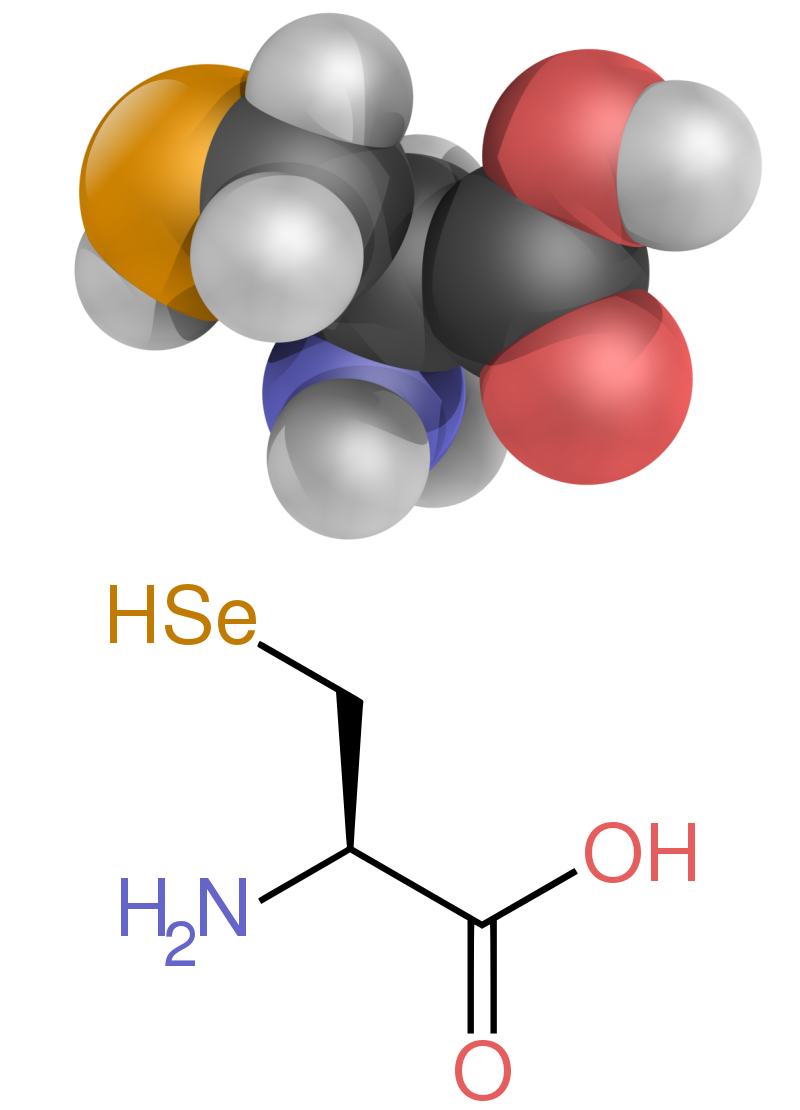
\includegraphics[width=0.3\textwidth]{Immagini/800px-Selenocysteine_skeletal_3D.png}
    \caption{Esempio di amminoacido}
    \label{fig:Amminoacido}
\end{figure}

In biochimica, ci si riferisce di solito ad un sottogruppo dei seguenti, ovvero gli $L-\alpha-amminoacidi$, ovvero amminoacidi il cui gruppo amminico e carbossilico sono 
legati allo stesso atomo di carbonio, chiamato appunto $\alpha$ e la loro configurazione è ad L, ovvero il gruppo amminico si troverà sempre alla sinistra del carbonio $\alpha$.
Sono presenti 22 $L-\alpha-amminoacidi$ che costituiscono la struttura delle proteine, anche detti amminoacidi proteinogenici. 
Oltre hai al gruppo carbosillico e al gruppo aminico, ogni amminoacido si contraddistingue dagli altri per la presenza di un residuo R, conosciuto anche con il nome di 
catena laterale.

\begin{figure}
    \centering
    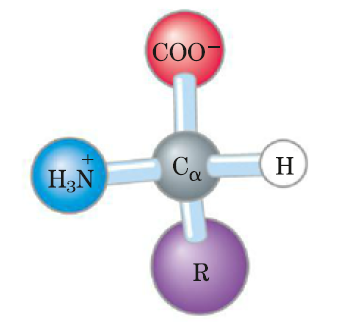
\includegraphics[width=0.4\textwidth]{Immagini/StrutturaAmminoacido.png}
    \caption{Struttura dell'amminoacido}
    \label{fig:AmminoacidoStruttura}
\end{figure}
\subsection{Catena laterale}\label{subsec:Catena_laterale}
La catena laterale gioca degli amminoacidi gioca un ruolo importante per la determinazione delle proprietà delle proteine. Esiste una vasta diversità nelle proprietà 
chimiche delle catene laterali degli amminoacidi, tuttavia essi possono essere raggruppati in 6 classi differenti.

\begin{table}[ht]
    \centering
    \resizebox{0.99\linewidth}{!}{
        \begin{tabular}{%
            |>{\itshape}p{40mm}%
            |>{\ttfamily}p{75mm}|}
            \hline
            Tipo di catena laterale & Amminoacidi \\
            \hline
            Alifatica & Glicina, alanina, valina, leucina, isoleucina\\
            \hline
            Contenente idrossile o solfuro & Serina, cisteina, treonina, metionina\\
            \hline
            Aromatica & Fenilalanina, tiroxina, triptofano\\
            \hline
            Basica & Istidina, lisina, arginina\\
            \hline
            Acido e la sua ammide & Acido aspartico, acido glutammico, asparagina, glutammina\\
            \hline
            Ciclica & Prolina\\
            \hline
        \end{tabular}
    }
    \vspace*{2mm}
	\caption{Classi di amminoacidi}
	\label{tab:tabellaclassiamminoacido}    
\end{table}

La prolina non può essere inserita in una qualsiasi classe perché è ciclica. La prolina condivide la maggior parte delle proprietà 
con i gruppi alifatici. La rigidità dell'anello gioca un ruolo cruciale nella struttura delle proteine. Come già detto, 
gli amminoacidi sono i mattoni di costruzione delle proteine e la metà di questi sono anche essenziali per l'essere umano, 
poiché non è in grado di produrseli da soli.  

Gli amminoacidi in azione combinata o in azione singola sono alla base di molte attività presenti nel nostro corpo.
%%% Valuta se inserire le caratteristiche peculiari degli amminoacidi


\section{Proteine}\label{sec:cap_sec_subsec}
Le informazioni trattate in questa sezione sono prese da \cite{WikiProteine}
A livello chimico, le proteine non sono altro che macromolecole biologiche costituite da catene di amminoacidi legate insieme da un legame peptidico. Il legame 
peptidico o giunto peptidico è un legame covalente che unisce il gruppo (-NH\_2) di un amminoacido con il gruppo (-COOH) di un altro amminoacido. Negli organismi 
viventi le proteine svolgono innumerevoli funzioni, tra cui la catalisi delle reazioni metaboliche, funzione di sintesi come replicazione del DNA, la risposta a 
stimoli e il trasporto di molecole da un luogo ad un altro. Le proteine in generale si differiscono nella sequenza degli amminoacidi, che viene conservata nei geni 
e che si traduce in un particolare ripiegamento della stessa e una struttura tridimensionale specifica che caratterizza la sua attività.

A differenza di altre macromolecole biologiche come i polisaccaridi e gli acidi nucleici, le proteine sono essenziali negli organismi viventi perché prendono parte 
a praticamente tutti i processi che avvengono nelle cellule. La maggior parte appartiene alla categoria degli enzimi, che caratterizzano le reazioni biochimiche 
vitali per il metabolismo degli organismi. Hanno anche funzioni strutturali o meccaniche nei muscoli e che costituiscono il citoscheletro. Alcune sono fondamentali 
per l'invio di segnali inter ed intracellulari e nella difesa immunitaria. Una volta che sono sintetizzate all'interno del organismo, esistono per un periodo di 
tempo limitato per poi esser degradate e riciclate attraverso meccanismi cellulari. 

Le proteine possono essere purificate da altri componenti cellulari e utilizzando tecniche come: l'ultracentrifugazione; la precipitazione; l'elettroforesi; 
la cromatografia. L'avvento dell'ingengneria genetica ha portato a nuove tecniche che ne facilitano la purificazione. 

Una catena lineare di residui amminoacidi è chiamata polipeptide, ed una proteina generalmente è costituita da uno o più polipeptidi lunghi eventualmente coordinati 
a gruppi non peptidici, chiamati prostetici o cofattori. I polipeptidi che contengono meno di 20/30 amminoacidi non vengono quasi mai considerati proteine, ma più 
spesso chiamati peptidi. La sequenza degli amminoacidi in una proteina è definita della sequenza presente nel gene a sua volta codificata nel codice genetico, 
solitamente ne sono specificati 20 ma possono essere di più in alcuni organismi.

Le proteine che hanno stesso numero e tipo di amminoacidi possono differire per come vengono posti all'interno della struttura, anche una singola variazione può 
portare ad una variazione nella struttura tridimensionale della macromolecola che può rendere la proteina non funzionale. 

\subsection{Classificazione}\label{subsec:es_subsec}

Durante l'evoluzione ci sono stati duplicamenti di geni e alterazioni della funzione di una proteina che portano tutt'ora ad avere circa 500 famiglie proteiche. 
All'interno della stessa famiglia le proteine svolgono funzioni leggermente diverse, ma per quanto riguarda la loro composizione a livello di sequenza di amminoacidi
è quasi identica. Chiaramente ci sono anche casi in cui le proteine all'interno della stessa famiglia si differiscono a livello di sequenza di amminoacidi, ma hanno 
una conformazione tridimensionale molto simile. 

Si afferma quindi che nel corso dell'evoluzione si sia più conservata la conformazione tridimensionale, piuttosto che la sequenza. Si può dire che due proteine hanno 
la stessa struttura generale quando almeno un quarto della loro sequenza amminoacidi corrisponde. Si dice invece che due proteine hanno un qualche grado di parentela, 
se almeno il 30\% degli amminoacidi corrisponde. Alcune proteine possono anche essersi formate per rimescolamento dei domini proteici o per la duplicazione 
all'interno della proteina stessa con unioni accidentali di DNA. 

La classificazione può essere ottenuta grazie alla composizione chimica, alla configurazione molecolare o alla solubilità. Ci sono quindi proteine semplici che 
sono costituite da soli amminoacidi e proteine coniugate composte dalla proteina semplice e da un gruppo prostetico non proteico.

Tra le proteine semplici vi sono le proteine fibrose, tendenzialmente non solubili nei solventi acquosi e poco attaccabili dagli enzimi proteolitici, inoltre sono
presenti le proteine globulari. Mentre per quanto riguarda le proteine coniugate troviamo l'emoglobina, le clorofille e le opsine.

Si possono poi classificare le proteine in base alla funzione che compiono, ci sono le proteine strutturali che sono componenti delle strutture permanenti e che 
hanno funzione meccanica, poi trovano posto le proteine di trasporto che prendono le sostanza poco idrosolubili e ne consentono il trasporto nell'organismo e poi
trovano posto gli enzimi che sono proteine catalitiche. A queste funzioni che abbiamo brevemente descritto si aggiugono la regolazione dell'espressione dei geni, 
la duplicazione, trascrizione e traduzione del DNA, la regolazione delle reazioni metaboliche, la generazione e la ricezione degli impulsi nervosi. 

\subsection{biochimica}\label{subsec:es_subsec}

La stra grande maggioranza delle proteine sono costituite da polimeri lineari combinando 20 diversi $L-\alpha-amminoacidi$. Tutti gli aminoacidi che possono essere 
impiegati nella costruzione di proteine hanno una struttura comune, un carbonio $\alpha$ con un gruppo amminico, un gruppo carbosillico e una catena laterale 
variabile a seconda dell'aminoacido, l'unica che si distingue è la prolina che contiene un anello insolito al gruppo amminico. Le catene laterali degli amminoacidi 
hanno ognuna la loro struttura e le loro proprietà chimiche, l'effetto combinato delle catene laterali determina la struttura tridimensionale e la reattività chimica
della proteina. Una volta collegati tramite legame peptidico gli amminoacidi sono chiamati residui e la serie di carbonio, azoto e atomi d'ossigeno è nota come 
catena principale o backbone.

Il legame peptidico ha due forme di risonanza che contribuiscono al doppio legame e non permettono la rotazione attorno al suo asse, in modo tale che i carbonio 
$\alpha$ dei vari residui siano pressoche complanari. Ci sono però altri due angoli nel legame peptidico che ne determinano la forma assunta. 

\subsection{Composizione}\label{subsec:es_subsec}
Uno dei dogmi fondamentali della biologia è che ad ogni struttura tridimensionale di una proteina via sia associata una specifica funzione biochimica. In questo modo
le proteine possono essere classificate in due famiglie: le proteine globulari e le proteine a struttura estesa o fibrosa. Questa separazione riflette anche una
separazione funzionale:
\vspace{10pt}
\begin{itemize}
    \item le proteine estese o fibrose svolgono funzioni biomeccaniche quindi fornendo sostegno strutturale;
    \vspace{5pt}
    \item le proteine globulari sono coinvolte in molteplici e specifiche funzioni biologiche e sono di fondamentale importanza per l'economia cellulare.
\end{itemize}

Una proteina è formata da uno o più polipeptidi, che sono molecole con più di 10 unità di amminoacidi, eventualmente accompagnati o legati da uno o più gruppi
prostetici. Una proteina attiva può esistere solo in soluzioni salina diluita e la sua struttura dipendera esclusivamente dalle caratteristiche chimico-fisiche
della soluzione in cui è inserita, che può anche determinare modifiche strutturali e alterare le sue propieta funzionali. 

La molecola proteica risulta costituita da atomi di carbonio, ossigeno, idrogeno e azoto, può contenere anche zolfo  e, talvolta, fosforo e/o metalli.

\subsection{Struttura}\label{subsec:es_subsec}
Mettiamo un sunto sensato delle sottosottosezioni....
\subsubsection{Ripiegamento}\label{subsec:es_subsec}
Prendendo una proteina, ovvero una macromolecola formata da decina di migliaia di atomi, potrebbe assumere un numero di ripiegamenti elevati; tuttavia, non è 
cosi perché ci sono considerazioni fisiche che limitano la maggior parte dei ripiegamenti. Gli atomi non possono sovrapporsi e il loro comportamento è da immaginarsi
come delle semplici sfere, con un certo raggio detto raggio di van der Waals. Ciascun amminoacido contribuisce alla formazione della catena con tre possibili legami:
\vspace{10pt}
\begin{itemize}
    \item legame peptidico (C-N) tra il carbonio di un amminoacido e l'azoto di un amminoacido adiacente;
    \vspace{5pt}
    \item legame convezionalmente chiamato C$\alpha$-C che è presente nei due carboni della catena principale del singolo amminoacido;
    \vspace{5pt}
    \item legame C$\alpha$-N all'interno dello stesso amminoacido.
\end{itemize} 

Il legame peptidico è planare e non consente alcuna rotazione, mentre gli altri due legami possono ruotare e definiscono due angoli: l'angolo di rotazione del 
legame C$\alpha$-C è detto $\psi$; l'angolo di rotazione del legame C$\alpha$-N è $\varphi$. La conformazione degli atomi che fanno parte della catena principale 
è determinata dagli angoli descritti in precedenza. Non è pero possibile ruotare come si vuole questi angoli dato che non sono possibili collisioni steriche tra gli 
amminoacidi. Ramachandran come vedremo nella prossima sezione nel dettaglio ha individuato e rappresentato in un grafico le coppie di angoli di rotazione a seconda
delle coppie di atomi. Dal grafico si può vedere che le proteine assumono due grandi tipologie di conformazione: l'$\alpha-elica$ e il $\beta-foglietto$.

Tra gli atomi che sono all'interno di una proteina si stabiliscono dei legami che possono essere covalenti o non covalenti, i legami non covalenti sono sicuramente 
meno potenti, tuttavia il numero all'internoo di una proteina li rende fondamentali per comprendere il ripiegamento. Ci sono tre tipi di legami non covalenti:
\vspace{10pt}
\begin{itemize}
    \item il legame idrogeno, che si effettua tra un atomo di ossigeno e uno vicino ad idrogeno;
    \vspace{5pt}
    \item le attrazzioni elettrostatiche che avvengono tra gruppi laterali con cariche periferiche opposte;
    \vspace{5pt}
    \item le attrazzioni di van der Waals si verificano tra dipoli molecola istantanei indotti, tra dipoli permanenti o tra un dipolo permanente e uno corrisponde 
    indotto, nelle quali entrano in gioco forze diverse.
\end{itemize} 

Vanno aggiunte alle precendenti interazioni la tendenza dei gruppo di amminoacidi idrofobici ad avvicinarsi e unirsi tra loro, formando delle tasche idrofobiche che
sono però lontane dai legami idrogeno sempre presenti in un ambiente acquoso. Tendenzialmente questi gruppi sono posti all'interno della proteina, mentre i suoi 
amminoacidi idrofili (polari e con carica) saranno tendenzialmente all'esterno, poiché essa si trova tipicamente in un ambiente acquoso. Di solito la proteina 
tende poi ad assumere la struttura tridimensionale che ha la più bassa energia libera.

\subsubsection{Le conformazioni più comuni}\label{subsec:es_subsec}
L'$\alpha-elica$ e il $\beta-foglietto$ sono le conformazioni più comuni riscontrabili nelle catene polipeptidiche di una proteina. Una singola proteina può 
prevedere sia $\alpha-elica$ che $\beta-foglietto$ in numero variabile.

L'$\alpha-elica$ è la più comune nelle proteine, in particolare nei recettori cellulari, e si possono trovare più $\alpha-elica$ per singola proteina. L'elica è 
una delle conformazioni più favorevoli perché riduce al minimo l'energia libera. Essa si forma quando una catena polipeptidica si ripiega su se stessa con formazione
di legami idrogeno tra un legame peptidico e il quarto successivo, nel dettaglio tra il gruppo chetonico C=O dell'uno e il gruppo N-H dell'altro, e il legame 
è tra O e H. Tutti i gruppi amminici di un'elica sono rivolti verso l'N-terminale della proteina, tutti quelli chetonici verso il C-terminale, così l'elica assume 
parziale carica positiva all'N-terminale e parziale carica negativa al C-terminale.

Il $\beta-foglio$ pieghettato è la seconda conformazione più comune nelle proteine, si trova maggiormente in alcuni enzimi e nelle proteine coinvolte nella difesa 
immunitaria. Esso consiste in numerose catene polipeptidiche che si dispongono l'una adiacente all'altra, collegate in una struttura continua da brevi sequenze ad U.

\subsubsection{Livelli di organizzazione}\label{subsec:es_subsec}
All'interno della proteina si possono distinguere vari livelli di organizzazione, che possono essere tre o quattro a seconda della tipologia della stessa.
I livelli d'organizzazione sono: 
\vspace{10pt}
\begin{itemize}
    \item la struttura primaria è formata dalla sequenza specifica di amminoacidi, dalla catena peptidica e il numero delle catene determina anche il ripiegamento
    della stessa;
    \vspace{5pt}
    \item la struttura secondaria consiste nella conformazione delle catene ($\alpha-elica$, $\beta-foglietto$, etc..). All'interno di una singola proteina vi può 
    essere una combinazione una combinazione di varie tipologie di sequenze;
    \vspace{5pt}
    \item il dominio è un'unità globulare o fibrosa formata da catene polipeptidiche ripiegate in più regioni compatte, costituiscono divisioni della struttura 
    terziaria, ha la caratteristica di ripiegarsi più o meno indipendentemente rispetto al resto della proteina. Molte delle proteine più complesse sono 
    aggregazioni modulari di numerosi dominii proteici;
    \vspace{5pt} 
    \item la struttura terziaria, che dal punto di vista termodinamo è quella ccon la più bassa energia libera, è rappresentata dalla configurazione tridimensionale
    completa che la catena polipeptidica assume nell'ambiente in cui si trova;
    \vspace{5pt}
    \item la struttura quaternaria deriva dall'associazione di due o più unità polipeptidiche, unite tra loro da legami deboli.
\end{itemize} 

Le proteine contenenti una parte non polipeptidica sono anche dette coniugate. Due proteine possono essere definite isoforme se a parità di struttura primaria ci sono 
differenze in uno degli altri livelli di struttura. Quando si dice denaturare una proteina significa distruggerne la sua conformazione spaziale, anche se viene 
mantenuta intatta la struttura primaria, essa non è più in grado di esplicare la sua funzione.

\subsubsection{Proteine complesse}\label{subsec:es_subsec}
Le proteine prese singolarmente sono si complesse, ma all'intermo degli organismi possono aggregarsi ad altre proteine identiche e non creando cosi dei complessi
proteici. Tutto ciò avviene grazie ai legami non covalenti che permettono ad una proteina di assumere una determinata configurazione. Nella proteina sono presenti 
una o più zone capaci di interazioni covalenti e vengono chiamate sidi di legame. Quando le proteine si uniscono insieme in un complesso proteico, le singole unità 
vengono chiamate subunità proteiche.

Ci sono complessi proteici formati da molte subunità che permettono di realizzare filamenti, poiché in un polo possiedono un sito di legame e dall'altro una struttura
proteica complementare allo stesso sito. Vi sono poi proteine la cui funzione è resa possibile proprio dalla loro struttura poco caratterizzabile e quasi casuale;
esse principalmente hanno molte funzioni all'interno della cellula. La loro caratteristica è quella di avere ridondanza di amminoacidi e bassa presenza di 
amminoacidi idrofobici. 

Ci possono essere casi in cui la proteina è esposta ad un alto livello di degradazione, esse sono quindi stabilizzate da legami di solfuro, che permettono di 
mantenere la sua conformazione.

\section{Principio di Ramachandran}\label{sec:cap_sec_subsec}
Le informazioni trattate in questa sezione sono prese da \cite{SlideRamachandran} e da \cite{TutorialRamachandran}.
Come detto nella sezione precedente Phi $\varphi$ e Psi $\psi$ determinano la conformazione di un polipeptide. Il principio di Ramachandran ci dice quali $\alpha-elica$, 
$\beta-foglietto$ e spire sono le conformazioni più probabili da adottare per una catena polipeptidica, poiché la maggior parte delle configurazioni sono 
impossibili a causa delle collisioni steriche tra gli atomi. 

\begin{figure}
    \centering
    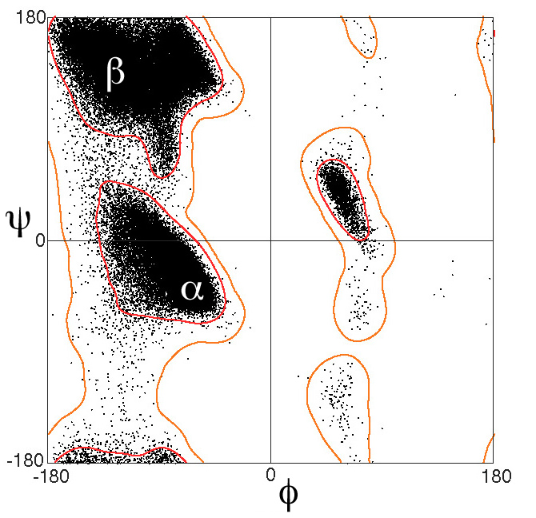
\includegraphics[width=0.4\textwidth]{Immagini/GraficoRamachandran.png}
    \caption{Esempio del grafico di Ramachandran}
    \label{fig:graficoRamachandran}
\end{figure}

Il principio di Ramachandran ha stabilito che solo alcune configurazioni di angoli di torsione sono stabili e presenti naturalmente nelle proteine. 
Queste configurazioni stabili sono descritte come regioni favorevoli o regioni accettabili nel grafico di Ramachandran. Le configurazioni non favorevoli o 
non accettabili sono associate con strutture instabili o anomale.

Il principio di Ramachandran viene utilizzato nella biologia strutturale per verificare la qualità delle predizioni di struttura proteica e per identificare 
eventuali errore nella modellizzazione. Viene anche utilizzato nella progettazione di proteine artificiali e nella modifica della struttura delle proteine 
esistenti per migliorare le proprietà terapeutiche o funzionali.

Non tutte le coppie di angoli teoricamente possibili sono realmente ottenibili all'interno delle strutture peptidiche in quanto impedite dalla presenza di 
ingombri sterici fra i gruppi delle catene laterali dei residui amminoacidici; le zone del grafico in cui tali contatti sterici sfavorevoli non sono presenti 
possono essere delimitate da linee di contorno, e possono essere associate ai motivi secondari assunti dalla catena. La conformazione complessiva del peptide 
è quindi definita assegnando i valori a ciascuna coppia di angoli $\psi$i, $\varphi$i per ogni amminoacido.

Nel caso della glicina, le zone di conformazioni possibili nel grafico presentano una simmetria centrale e sono molto più ampie rispetto a quelle degli 
altri amminoacidi grazie alla simmetria del residuo ed alle piccole dimensioni dell'atomo di idrogeno legato in posizione $\alpha$. Gli altri amminoacidi presentano 
invece un diagramma asimmetrico, con un insieme di zone indicanti le conformazioni ammesse meno esteso, e la cui ampiezza dipende soprattutto dalla presenza 
di gruppi stericamente ingombranti in posizione $\beta$. La presenza di catene laterali, anche lunghe, che non siano ramificate al carbonio $\beta$, come nel caso della 
leucina, ha invece una scarsa influenza e riduce solo di poco il dominio delle conformazioni permesse.

Un caso a parte si ha per la prolina, la cui struttura rigida rende possibili solo poche conformazioni in una porzione limitata del grafico.

\section{Ricerca Locale}\label{sec:cap_sec_subsec}
La ricerca locale è una tecnica euristica di ottimizzazione e risoluzione dei problemi che mira a trovare una soluzione che sia vicina alla soluzione attuale e la migliori. 
Funziona apportando piccole modifiche alla soluzione corrente e valutando i risultati, con l'obiettivo di trovare una soluzione ottimale in uno spazio di ricerca 
limitato. La ricerca locale viene spesso utilizzata nei problemi di ottimizzazione combinatoria, come il problema del commesso viaggiatore, e nell'apprendimento 
automatico, dove può essere utilizzata per ottimizzare algoritmi complessi come le reti neurali. L'idea chiave alla base della ricerca locale è evitare di rimanere 
bloccati in soluzioni non ottimali apportando una serie di piccole modifiche informate alla soluzione corrente fino a quando non viene trovata una soluzione ottimale.

La ricerca locale è un sottocampo di:
\vspace{10pt}
\begin{itemize}
    \item Metaheuristic: è una procedura o euristica di livello superiore progettata per trovare, generare o selezionare un'euristica che può fornire una soluzione
    sufficientemente buona a un problema di ottimizzazione, in particolari con informazioni incomplete o limitate capacità di calcolo;
    \vspace{5pt}
    \item Stochastic optimization: sono metodi di ottimizzazione che generano e utilizzano variabili casuali; I metodi di ottimizzazione stocastica generalizzano metodi 
    deterministici per problemi deterministici;
    \vspace{5pt}
    \item Mathematical optimization: è la selezione di un elemento migliore rispetto ad un qualche criterio, da un insieme di alternative disponibili; Nell'approccio 
    più generale, un problema di ottimizzazione consiste nel massimizzare o minimizzare una funzione reale scegliendo sistematicamente i valori di input 
    all'interno di un insieme consentito e calcolando il valore della funzione.
\end{itemize}

La maggior parte dei problemi può essere formulata in termini di spazio di ricerca e target in diversi modi. Ad esempio, per il problema del commesso viaggiatore una 
soluzione può essere un percorso che tocca tutte le città e l'obiettivo è trovare il percorso più breve. Ma una soluzione può anche essere un percorso, che può anche 
contenere un ciclo.

Un algoritmo di ricerca locale parte da una soluzione candidata e quindi si sposta iterativamente verso una soluzione vicina; un quartiere è l'insieme di tutte le 
possibili soluzioni che differiscono dalla soluzione attuale per la minima misura possibile. Ciò richiede la definizione di una relazione di vicinato nello spazio 
di ricerca. Ad esempio, l'intorno della copertura del vertice è un'altra copertura del vertice che differisce solo per un nodo. Per la soddisfacibilità booleana, 
i vicini di un'assegnazione booleana sono quelli che hanno una singola variabile in uno stato opposto. Lo stesso problema può avere più quartieri distinti definiti 
su di esso; l'ottimizzazione locale con quartieri che implicano la modifica di fino a k componenti della soluzione viene spesso definita k-opt.

Tipicamente, ogni soluzione candidata ha più di una soluzione vicina; la scelta di quale selezionare viene presa utilizzando solo le informazioni sulle soluzioni 
nelle vicinanze dell'assegnazione corrente, da cui il nome ricerca locale. Quando la scelta della soluzione del vicino è fatta prendendo quella che massimizza 
localmente il criterio, cioè: una ricerca avida, la metaeuristica prende il nome di hill climbing. Quando non sono presenti vicini in miglioramento, 
la ricerca locale è bloccata in un punto localmente ottimale. Questo problema di ottimo locale può essere risolto utilizzando i riavvii (ricerca locale ripetuta 
con diverse condizioni iniziali), la randomizzazione o schemi più complessi basati su iterazioni, come la ricerca locale iterata, sulla memoria, come 
l'ottimizzazione della ricerca reattiva, su modifiche stocastiche senza memoria, come la simulated annealing.

La ricerca locale non fornisce una garanzia che una determinata soluzione sia ottimale. La ricerca può terminare dopo un determinato periodo di tempo o quando la 
migliore soluzione trovata fino a quel momento non è migliorata in un determinato numero di passaggi. La ricerca locale è un algoritmo anytime: può restituire 
una soluzione valida anche se viene interrotta in qualsiasi momento dopo aver trovato la prima soluzione valida. La ricerca locale è in genere un'approssimazione 
o un algoritmo incompleto, poiché la ricerca potrebbe interrompersi anche se la migliore soluzione corrente trovata non è ottimale. Ciò può accadere anche se 
la terminazione avviene perché la migliore soluzione attuale non può essere migliorata, poiché la soluzione ottima può trovarsi lontano dall'intorno delle 
soluzioni attraversate dall'algoritmo.

Schuurman \& Southey propongono tre misure di efficacia per la ricerca locale (profondità, mobilità e copertura):
\vspace{10pt}
\begin{itemize}
    \item Profondità: il costo dell'attuale (migliore) soluzione;
    \vspace{5pt}
    \item Mobilità: la capacità di spostarsi rapidamente in diverse aree dello spazio di ricerca (mantenendo bassi i costi);
    \vspace{5pt}
    \item Copertura: quanto sistematicamente la ricerca copre lo spazio di ricerca, la distanza massima tra qualsiasi incarico inesplorato e tutti gli incarichi
    visitati.
\end{itemize}

Ipotizzano che gli algoritmi di ricerca locale funzionino bene, non perché abbiano una certa comprensione dello spazio di ricerca, ma perché si spostano 
rapidamente in regioni promettenti ed esplorano lo spazio di ricerca a basse profondità nel modo più rapido, ampio e sistematico possibile.

\subsection{Tipologie di ricerca locale}\label{subsec:es_subsec}
La ricerca locale si basa sul presupposto che il miglioramento di una soluzione che si trovi nelle immediate vicinanze di quest'ultima (vicinato).
Data una qualsiasi soluzione euristica (nodo corrente) la ricerca locale verifica l'esistenza di soluzioni migliori nell'insieme delle soluzioni più vicine 
(nodi vicini). Ad esempio, un algoritmo di ricerca locale può essere utilizzato per risolvere il problema del commesso viaggiatore. 
Le tecniche di ricerca locale consentono di raggiungere risultati sia nella ricerca delle soluzioni a un problema (problem solving) e sia 
nell'ottimizzazione. Appartengono alla categoria degli algoritmi di ricerca locale i seguenti algoritmi:
\begin{itemize}
    \item Ricerca hill climbing: L'algoritmo di ricerca hill climbing è una tecnica di ricerca locale in cui il nodo corrente è sostituito con il nodo migliore;
    \vspace{5pt}
    \item Simulated annealing: L'algoritmo di Simulated annealing o Annealing simulato (SA) è un algoritmo probabilistico-metaeuristico di ottimizzazione 
    della ricerca in uno spazio di ricerca di grandi dimensioni. Il suo nome prende spunto dal processo metallurgico che consente di riaggregare la materia fusa 
    dei metalli in base a determinate caratteristiche comuni. Nell'algoritmo di simulated annealing un processo di selezione consente l'eventuale sostituzione 
    della soluzione del nodo corrente con quella di un nodo selezionato casualmente da una lista di soluzioni candidate;
    \vspace{5pt}
    \item Beam Search. La beam search è una ricerca locale basata su tecniche euristiche. La beam search ( ricerca di fascio ) esplora un fascio limitato di 
    nodi promettenti (soluzioni parziali) dello spazio di ricerca e li analizza con una ricerca locale. Utilizzando le tecniche euristiche l'algoritmo beam search 
    consente di riconoscere quando una soluzione parziale è anche una soluzione completa.
\end{itemize}



\subsection{Euristiche}\label{subsec:es_subsec}
Un algoritmo di tipo Ricerca Locale appartengono alla classe delle euristiche di miglioramento. Sono euristici quegli algoritmi che non garantiscono di fornire 
la soluzione ottima. Ovvero, data una soluzione iniziale ammissibile s, essa è migliorata attraverso successive trasformazioni di s.

Le euristiche sono quindi strategie che aiutano a trovare una soluzione ottimale in una ricerca locale. Ecco alcune delle eurisiche più comuni utilizzate nella 
ricerca locale:
\vspace{10pt}
\begin{itemize}
    \item First-Improvement: Questa euristica cerca sempre la prima soluzione migliore rispetto alla soluzione corrente. Il vantaggio di questa euristica è 
    che è molto veloce, poiché interrompe la ricerca non appena viene trovata una soluzione migliore. Tuttavia, il suo limite è che potrebbe non essere in 
    grado di trovare la soluzione ottimale, poiché potrebbe fermarsi presto;
    \vspace{5pt}
    \item Best-Improvement: Questa euristica cerca sempre la migliore soluzione possibile rispetto alla soluzione corrente. Il vantaggio di questa euristica 
    è che è molto precisa, poiché cerca sempre la soluzione migliore. Tuttavia, il suo limite è che potrebbe essere molto lenta, poiché deve valutare 
    tutte le soluzioni possibili prima di scegliere la migliore;
    \vspace{5pt}
    \item Stochastic Hill Climbing: Questa euristica cerca una soluzione migliore casualmente. Il vantaggio di questa euristica è che è molto flessibile, 
    poiché cerca soluzioni in modo casuale. Tuttavia, il suo limite è che potrebbe essere impreciso, poiché potrebbe scegliere soluzioni subottimali;
    \vspace{5pt}
    \item Simulated Annealing: Questa euristica cerca una soluzione migliore basata sulla probabilità. Il vantaggio di questa euristica è che è molto 
    precisa, poiché cerca soluzioni basate sulla probabilità. Tuttavia, il suo limite è che potrebbe essere molto lenta, poiché deve valutare molte 
    soluzioni prima di scegliere la soluzione migliore;
    \vspace{5pt}
    \item Variable Neighborhood Search: Questa euristica cerca soluzioni migliori cambiando continuamente il vicinato della soluzione corrente. Il vantaggio 
    di questa euristica è che è molto flessibile, poiché cerca soluzioni in molti vicinati diversi. Tuttavia, il suo limite è che potrebbe essere molto lenta, 
    poiché deve valutare molte soluzioni prima di scegliere la soluzione migliore;
    \vspace{5pt}
    \item Greedy Algorithm: Questa euristica seleziona sempre la soluzione che sembra essere la migliore in un determinato momento. Il vantaggio di questa 
    euristica è che è molto veloce, poiché seleziona sempre la soluzione migliore. Tuttavia, il suo limite è che potrebbe non essere in grado di trovare la 
    soluzione ottimale, poiché seleziona sempre la soluzione migliore in un dato momento, senza preoccuparsi delle conseguenze future. Pertanto, 
    è importante utilizzare questo algoritmo con cautela e verificare che la soluzione ottenuta soddisfi i requisiti del problema.
\end{itemize}

\section{Hydropathic INTeractions HINT}\label{sec:cap_sec_subsec}
% File preso da Federica Agosta https://link.springer.com/article/10.1007/s10822-022-00477-y
%https://it.wikipedia.org/wiki/Forza_intramolecolare
Le informazioni trattate in questa sezione sono prese da \cite{AgostaCozzini} e da \cite{ForzaIntramolecolare}.
La valutazione della stabilità intramolecolare di una proteina gioca un ruolo fondamentale nella comprensione del loro comportamento e nel meccanismo di azione. Piccole alterazioni strutturali possono impattare l'attività biologica e di conseguenza la modulazione farmacologica. 
L'analisi della struttura tridimensionale della proteina e la risultante stabilità permettono di predirre un possibile meccanismo di attivazione e rivelano nuove strategie per scoprire nuovi farmaci. Ogni modifica apportata alla struttura di una proteina porta quasi sicuramente ad una variazione del suo meccanismo di azione, e valutare la stabilità di una proteina mutata può essere molto costoso in termini di tempo.
La stabilità delle proteine mutate è influenzata dall'interazione intramolecolare, ovvero sono forze che permettono di creare e tenere insieme una struttura. Nel tentativo di analizzare la stabilità proteica, sono stati sviluppati molti metodi che svariano in diversi approcci dai meccanismi molecolari basati su force field fino a tecniche di machine learning. Tuttavia, questa pratica risulta essere molto costosa, specialmente quando sono presenti un elevato numero di mutazioni. Uno degli aspetti fondamentali su cui è basato HINT è dovuta al fatto che la stabilità delle proteine mutate è dimostrato essere influenzata dalle interazioni intramolecolari. Le strutture native delle proteine sono relativamente stabili poiché si formano come risultato di un equilibrio tra le varie forze non covalenti a cui sono soggette: i legami idrogeno, i legami ionici, le forze di Wan der Walls e le interazioni idrofobiche. In generale le interazioni chimiche deboli sono attrazzioni tra atomi appartenenti o alla stessa molecola (intramolecolari) o a molecole diverse (intermolecolari). A differenza dei legami covalenti che legano gli atomi tra loro, le interazioni chimiche deboli non sono forti abbastanza per legare tra loro atomi isolati. Per questo le interazioni chimiche deboli si formano e si rompono in continuazione alla temperatura fisiologica dell'organismo. a meno che, cumulandosi in gran numero, esse non diano collettivamente stabilità alle strutture che contribuiscono a generare.

HINT è stato sviluppato sulla base dei lavoro svolto da (indica il personaggio) che ha esteso il metodo fragment per la predizione dei $\log P\_o/v$ (coefficiente di partizione per il trasferimento di soluti in 1-ottanolo/acqua), cio permette di quantificare le interazioni idrofobiche e polari tra o all'interno dei molecole. La funzione di energia intramolecolare di HINT può essere calcolata rapidamente dalla struttura in termini di somma di punteggi d'interazione atomo-atomo. Il punteggio intramolecolare viene calcolato come somma delle interazioni idrofobiche e polari tra tutte le coppie di atomi considerando l'area accessibile al solvente. Le interazioni idrofobiche si verificano quando le molecole non polari si avvicinano tra di loro in un solvente polare, come l'acqua. Le molecole non polari tendono a respingersi reciprocamente e ad attirarsi con le molecole del solvente. Il processo anche noto come esclusione dei solventi, porta alla formazioni di molecole non polari all'interno del solvente. Le molecole non polari quindi cercano di organizzarsi in modo tale da minimizzare il contatto con il solvente e massimizzare le interazioni tra di loro. 

Il punteggio energetico di HINT intramolecolare consente quindi di calcolare tutte le interazioni idropatiche (idrofobiche e polari) che si verificano nella molecola e ne consentono di valutare la stabilità termodinamica. Dato il suo livello di sensibilità nell'individuare piccole differenze di energie verrà poi utilizzato per stimare la stabilità della Glicoproteina spike del SARS-CoV-2.

\section{Shortest Path}\label{sec:cap_sec_subsec}
Lo shortest path è un importante concetto nell'ambito dell'informatica cosi come nell'ingegneria e nella matematica applicata. Essa si riferisce al percorso più
breve tra due punti in un grafo, ovvero insieme di nodi collegati da archi. 

Esso è molto importante per esempio nel campo della robotica, viene utilizzato per pianificare il percorso del robot, consentendogli di evitare ostacoli e
raggiungere il suo obiettivo in modo efficiente. Possiamo trovare lo stesso concetto applicato nelle reti di telecomunicazioni, poiché viene utilizzato per instradare
il traffico tra due nodi garantendo una comunicazione efficiente e affidabile. Viene anche usato in algoritmi di routing per cercare di minimizzare il tempo di ritardo.
Chiaramente esso si adatta bene nel campo della logistica dove è necessario ottimizzare il trasporto delle merci o delle persone. Infine, trova applicazione anche nel
campo della progettazione di circuiti elettronici.

\subsection{Algoritmo A*}\label{subsec:es_subsec}
L'algoritmo A* è spesso utilizzato nella risoluzione del problema dello shortest path, ovvero per trovare il percorso più breve tra due nodi in un grafo pesato. 
L'algoritmo A* utilizza una funzione di stima euristica per guidare la ricerca verso il percorso più breve, permettendo di ottenere un'efficace combinazione di completezza e velocità nell'individuare la soluzione.

Nella versione dello shortest path risolto con l'algoritmo A*, ogni nodo del grafo viene valutato in base alla sua distanza dal nodo di partenza, la stima della distanza dal nodo di arrivo e il costo totale del percorso, ovvero la somma della distanza dal nodo di partenza e della stima della distanza dal nodo di arrivo. In questo modo, l'algoritmo A* tiene traccia del percorso più breve scoperto fino a quel momento e lo utilizza per determinare quale nodo espandere successivamente.

L'algoritmo A* può essere ulteriormente ottimizzato attraverso l'utilizzo di tecniche come la memorizzazione della distanza minima calcolata per ogni nodo, in modo da ridurre il numero di espansioni necessarie. Inoltre, l'algoritmo A* può essere utilizzato con successo in grafi di grandi dimensioni, grazie alla sua capacità di selezionare le espansioni più promettenti e di escludere le aree meno promettenti del grafo.

\subsection{Esempio}\label{subsec:es_subsec}
In questo esempio, la funzione A\_star prende in input la cella di partenza 'start', la cella di arrivo 'goal' e una rappresentazione del labirinto come 'graph'. La funzione A\_star esplora le celle adiacenti alla cella corrente, calcola il costo del percorso per ogni cella e aggiunge le celle alla coda di priorità. La coda di priorità è ordinata in base al costo totale, che è la somma del costo del percorso e della stima euristica. La funzione A\_star restituisce il percorso più breve dal punto di partenza al punto di arrivo.

\begin{minipage}{\textwidth}
	\begin{lstlisting}[caption={Algoritmo A*}]
		# Definizione della funzione di costo
		def cost(current, next):
			if current[0] == next[0] or current[1] == next[1]:
				return 1
			else:
				return math.sqrt(2)
		
		# Definizione della funzione euristica
		def heuristic(current, goal):
			return math.sqrt((current[0]-goal[0])**2 + (current[1]-goal[1])**2)
		
		# Definizione dell'algoritmo A*
		def A_star(start, goal, graph):
			queue = []
			heapq.heappush(queue, (0, start, []))
			visited = set()
			
			while queue:
				_, current, path = heapq.heappop(queue)
				if current == goal:
				return path + [current]
				if current in visited:
					continue
				visited.add(current)
				for neighbor in graph[current]:
					if neighbor in visited:
						continue
					new_cost = cost(current, neighbor)
					total_cost = new_cost + heuristic(neighbor, goal)
					heapq.heappush(queue, (total_cost, neighbor, path + [current]))
			return None
	\end{lstlisting}
\end{minipage}

\section{Algebra e Geometria}\label{sec:algebra}
L'algebra e la geometria sono due aree fondamentali della matematica che sono strettamente correlate e si influenzano a vicenda. La geometria si occupa dello studio delle figure geometriche nello spazio, come punti, linee, piani, poligoni, solidi e curve. 

L'algebra, come accennato in precedenza, si occupa dello studio delle proprietà delle operazioni aritmetiche e delle relazioni tra le variabili. L'algebra fornisce uno strumento matematico molto potente per la risoluzione di problemi e l'espressione di relazioni matematiche in modo astratto.

L'algebra e la geometria sono strettamente correlate, poiché l'algebra può essere utilizzata per risolvere problemi geometrici, come ad esempio la determinazione di equazioni di rette e di superfici, la risoluzione di equazioni di secondo grado che descrivono curve, e la risoluzione di problemi di trigonometria.

D'altra parte, la geometria può essere utilizzata per visualizzare le relazioni algebriche, ad esempio rappresentando graficamente le funzioni algebriche o le equazioni differenziali.

\subsection{Spazio vettoriale}\label{subsec:spazi_vettoriali}
Gli spazi vettoriali sono una struttura algebrica complessa, composta da: un campo, in cui gli elementi sono detti scalari; un insieme, i cui elementi sono detti vettori; due operazioni binarie, la somma e la moltiplicazione scalare con determinate proprietà. 

Per ogni numero naturale $n \ge 1$ consideriamo l'insieme $\mathbf{R}^n$ delle n-uple ordinate di numeri reali: 

	$$\mathbf{R}^n = \{v = (x_1, .., x_n)| x_i \in \mathbf{R}\}$$.

Viene chiamato $\mathbf{R}^n$ lo spazio n-dimensionale e i suoi elementi vettori o punti. 
\begin{figure}
	\centering
	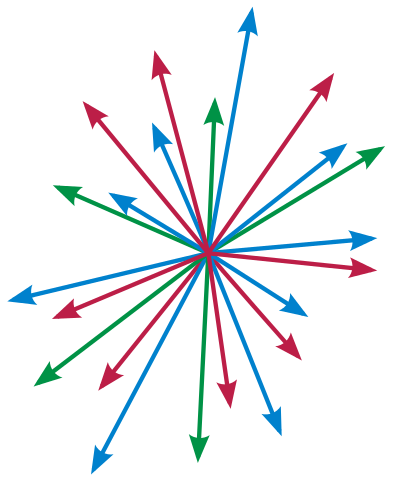
\includegraphics[width=0.3\textwidth]{Immagini/SpazioVettoriale.png}
	\caption{Uno spazio vettoriale è una collezione di oggetti, chiamati "vettori", che possono essere sommati e riscalati.}
	\label{fig:vettori}
\end{figure}
Presi due vettori $$v = (x_1, .., x_n) e w = (y_1, .., y_n)$$ si possono sommare componente per componente per ottenere un nuovo vettore: 

	$$v + w = (x_1 + y_1, .., x_n + y_n)$$.

Un numero $c \in \mathbf{R}$ si può moltiplicare con un vettore $v = (x_1, .., x_n)$ in modo da ottenere un nuovo vettore:

	$$cv = (cx_1, .., cx_n)$$.

Le operazioni di somma e moltiplicazione per scalare sono anche chiamate operazioni di spazio vettoriale. 

Per la somma di vettori $v, w, u \in \mathbf{R}$ vengono verificate le seguenti proprietà:
\vspace{10pt}
\begin{itemize}
	\item $v + w = w + v$;
	\vspace{5pt}
	\item $(v + w) + u = v + (w + u)$;
	\vspace{5pt}
	\item $v + \mathcal{O} = v, v + (-v) = \mathcal{O}$, dove $\mathcal{O} = (0, .., 0)$.
\end{itemize}

Per la moltiplicazione per scalare di $a, b \in \mathbf{R}$ con $v, w \in \mathbf{R}^n$ valgono invece: 
\vspace{10pt}
\begin{itemize}
	\item $a(bv) = (ab)v$;
	\vspace{5pt}
	\item $a(v + w) = av + aw, (a + b)v = av + bv$;
	\vspace{5pt}
	\item $1v = v$.
\end{itemize}
Si osserva che le operazioni di somma e di moltiplicazione per scalare si possono definire non solo nell'insieme dei numeri reali o delle n-uple di numeri, ma anche in altri insiemi (di funzioni, di matrici, ...). Un insieme con somma e moltiplicazione per scalare che verificano tutte le proprietà precedentemente descritte si dice spazio vettoriale.

\subsection{Prodotto scalare}\label{subsec:prodotto_scalare}
Il prodotto scalare di $v = (x_1, .., x_n) e w = (y_1, .., y_n)$ è il numero
	$$\langle v,w \rangle := x_1y_1 + x_2y_2 + ... + x_ny_n = \sum_{i=1}^{n} x_iy_i$$
talvolta viene anche denotato come $v \cdot w$. 

Ci sono importanti proprietà alla base del prodotto scalare, ovvero per $v, w, u \in \mathbf{R}^n e c \in \mathbf{R}$ valgono:
\vspace{10pt}
\begin{itemize}
	\item $\langle v,w \rangle = \langle w,v \rangle$;
	\vspace{5pt}
	\item $\langle v,w + u \rangle = \langle v,w \rangle + \langle v,u \rangle$;
	\vspace{5pt}
	\item $\langle cv,w \rangle = c\langle v,w \rangle = \langle v,cw \rangle$;
	\vspace{5pt}
	\item $\langle v,v \rangle \ge 0$, e $\langle v,v \rangle = 0 \iff v = \mathcal{O}$ (positività di $\langle , \rangle$).
\end{itemize}

Nel piano cartesiano il prodotto scalare permette di definire e trattare la nozione geometrica di lunghezza di un vettore. Tale concetto può essere esteso ad uno spazio vettoriale di dimensione arbitraria introducendo un concetto analogo: la norma. 

\subsection{Matrici di rotazione}\label{subsec:matrici_rotazione}
In matematica, e in particolare in geometria, una rotazione è una trasformazione del piano o dello spazio euclideo che sposta gli oggetti in modo rigido e che lascia fisso almeno un punto, nel caso del piano, o una retta, nel caso dello spazio. I punti che restano fissi nella trasformazione formano più in generale un sottospazio: quando questo insieme è un punto o una retta, si chiama rispettivamente il centro e l'asse della rotazione.

Più precisamente, una rotazione è una isometria di uno spazio euclideo che ne preserva l'orientazione, ed è descritta da una matrice ortogonale speciale. Qualunque sia il numero delle dimensioni dello spazio di rotazione, gli elementi della rotazione sono:
\vspace{10pt}
\begin{itemize}
	\item il verso (orario-antiorario);
	\vspace{5pt}
	\item l'ampiezza dell'angolo di rotazione;
	\vspace{5pt}
	\item l centro di rotazione (il punto attorno a cui avviene il movimento rotatorio).
\end{itemize}

Nel nostro caso ci concentriamo nello spazio a 3 dimensioni; in questo caso la rotazione è determinata da un asse, dato da una retta r passante per l'origine, e da un angolo $\theta$ di rotazione. Per evitare ambiguità, si fissa una direzione dell'asse, e si considera la rotazione di angolo $\theta$ effettuata in senso antiorario rispetto all'asse orientato. Senza cambiare base, la rotazione di un angolo $\theta$ intorno ad un asse determinato dal versore $(x, y, z)$ (ossia un vettore di modulo unitario) è descritta dalla matrice seguente:
$$
\begin{bmatrix}
	x^2+(1-x^2)\cos(\theta) & xy(1-\cos(\theta))-z\sin{\theta} & xz(1-\cos{\theta})+y\sin{\theta} \\
	xy(1-\cos(\theta))-z\sin{\theta} & y^2+(1-y^2)\cos(\theta) & yz(1-\cos{\theta})-x\sin{\theta} \\
	xz(1-\cos(\theta))-y\sin{\theta} & yz(1-\cos{\theta})+x\sin{\theta} & z^2+(1-z^2)\cos(\theta) \\
\end{bmatrix}
$$
Ponendo $(x, y, z) = (1, 0, 0)$ oppure $(x, y, z) = (0, 1, 0)$ oppure $(x, y, z) = (0, 0, 1)$ si ottiene rispettivamente la rotazione attorno all'asse $x$, all'asse $y$ e all'asse $z$. 
Tale matrice è stata ottenuta scrivendo la matrice associata alla trasformazione lineare (rispetto alle basi canoniche nel dominio e codominio) della formula di Rodrigues.

\subsection{Super Fibonacci Spirals}\label{subsec:superfibonaccispiral}
Le informazioni di questa sezione sono state recuperate da \cite{Alexa_2022_CVPR}.
Le super spirali di Fibonacci sono un'estensione delle spirali di Fibonacci che consentono la generazione rapida di un arbitrario ma fisso numero di orientamenti 3D. Una valutazione completa rispetto ad altri metodi mostra che gli insiemi di orientamenti generati hanno una bassa discrepanza, componenti spuri minimi nello spettro di potenza e volumi Voronoi quasi identici. 
L'ottimizzazione degli insiemi per discrepanze basse è difficile. Inoltre, l'ottimizzazione $\mathcal{SO}(3)$ è scomoda a causa della geometria sottostante. \footnote{$\mathcal{SO}(3)$ è il gruppo delle rotazioni tridimensionali che preservano la norma e il prodotto vettoriale, e che hanno determinante 1. Sono tutte le possibili rotazioni attorno ad un punto nello spazio tridimensionale, senza alcuna traslazione.}

Lo strumento principale per usare il campionamento di Fibonacci su $\mathcal{S}^3$ è una mappatura che preserva il volume di un cilindro solido in $\mathcal{R}^3$ alla 3-sfera. Considerando il cilindro ${(h, y = (y_0, y_1))| -\pi < h \le \pi, y^Ty \le 1}$. Allora 
$$
	x(h, y) = \begin{pmatrix}
				z \cos{h} \\
				z \sin{h} \\
				y_0 \\
				y_1  
			  \end{pmatrix}, z = \sqrt{1 - y^Ty}
$$
mappa punti nel cilindro della sfera $\mathcal{R}^4$. La mappatura inversa di $x = (x_0, x_1, x_2, x_3)$ è data da $(h, y_0, y_1) = (\arctan2(x_1,x_0),x_2,x_3)$. Questo mostra che la mappatura è una biezione tra l'interno relativo del cilindro e la sfera senza equatore $x_0 = x_1 = 0$. La linea ${-\pi < h \le \pi, y^Ty \le 1}$ sulla superficie del cilindro sono mappate ai punti $(0, 0, y_0, y_1)$ sull'equatore della sfera. All'interno del cilindro $y^Ty < 1$ dove la mappatura è biettiva, possiamo calcolare la Jacobians come: 
$$
	\mathcal{J}_{h, j} = \begin{pmatrix}
		-z\sin{h} -\frac{y_0}{z}\cos{h} -\frac{y_1}{z}\cos{h} \\
		z\cos{h} -\frac{y_0}{z}\sin{h} -\frac{y_1}{z}\sin{h} \\
		0 1 0 \\
		0 0 1 \\
	\end{pmatrix}
$$
Usando quindi Jacobians possiamo analizzare il cambio di volume e reclamare che la mappatura $x(h, y) = {(h, y)| -\pi < h \le \pi, y^Ty < 1} \mapsto \mathcal{S}^3 \subset \mathcal{R}^4$ preserva il volume. 

Si può dimostrare ciò che viene reclamato in precedenza come $det(x(h, y), J_(h, y))$, perché $x(h, y)$ è ortogonale alla tangente al piano e ha lunghezza unitaria. Sviluppando si ottiene

$$
	+z \cos{h}(z \cos{h}) - z \sin{h}(z \sin{h})
$$
$$
	+y_0 (y_0 \sin^2{h} + y_0 \cos^2{h}) 
$$
$$
	-y_1 (y_1 \cos^2{h} - y_1 \sin^2{h}) 
$$
$$
	= (1 - y^Ty)(\cos^2{h} + \sin^2{h}) + y^Ty = 1
$$.

Data la mappatura, l'idea è quella di utilizzare il campionamento di Fibonacci 2 volte per generare punti sul cilindro: la prima lungo l'asse principale $h$ del cilindro; la seconda sul cerchio $(y_0, y_1)$ ortogonale all'asse. Usando due differenti costanti $\phi$ e $\psi$, per i due campionamenti otteniamo:
$$
	y(t) = \bigg(\sqrt{t}\sin{\frac{2\pi nt}{\phi}}, \sqrt{t}\cos{\frac{2\pi nt}{\phi}} \bigg)
$$

$$
	z(t) = \bigg(\frac{nt}{\psi} - \biggl\lfloor\frac{nt}{\psi}\biggl\rfloor, \sqrt{t}\sin{\frac{2\pi nt}{\phi}}, \sqrt{t}\cos{\frac{2\pi nt}{\phi}}\bigg)^T
$$.

Inserendo questo campione nella mappatura della 3-sfera otteniamo la seguente semplice curva che esibisce la simmetria aspettata:
$$
w(t) = \begin{pmatrix}
	\sqrt{t}\sin{\frac{2\pi nt}{\phi}} \\
	\sqrt{t}\cos{\frac{2\pi nt}{\phi}} \\
	\sqrt{t-1}\sin{\frac{2\pi nt}{\psi}} \\
	\sqrt{t-1}\cos{\frac{2\pi nt}{\psi}} \\
\end{pmatrix}
$$.

Il campionamento di questa curva a valori regolari di $t_i$ è un metodo naturale per la generazione di campioni di orientamento. L'implementazione algoritmica è la seguente \ref{alg:sampling}.
\begin{algorithm}
	\caption{Generazione di n campioni in $\mathcal{SO}(3)$}\label{alg:sampling}
	\begin{algorithmic}
		\Function{Super-Fibonacci}{n, $\phi$, $\psi$} 
			\For{$i \in {0, .., n-1}$}
				 \State $s \gets i + \frac{1}{2}$
				 \State $t \gets \frac{s}{n}$, $d \gets 2\pi s$
				 \State $r \gets \sqrt{t}$, $R \gets \sqrt{1 - t}$
				 \State $\alpha \gets \frac{d}{\phi}$, $\beta \gets \frac{d}{\psi}$
				 \State $q_i \gets (r\sin{\alpha}, r\cos{\alpha}, R\sin{\beta}, R\cos{\beta})$
		    \EndFor
	    \EndFunction
	\end{algorithmic}
\end{algorithm}

Questo algoritmo mostra che un insieme di $kn$ campioni contiene l'insieme generato per $n$ campioni o, più generalmente, insieme con $m$ e $n$ campioni condividono ogni $k$-esimo campione, dove $k$ è il minimo comune diviso tra $m$ e $n$. Giocano un ruolo fondamentale anche gli altri due parametri di questo algoritmo, ovvero $\phi$ e $\psi$ che devono essere irrazionali, ma anche la loro relazione è importante. Non ci sono però teorie matematiche a supporto quindi è necessario adattarli alla situazione d'uso.

\chapter{Covid}\label{chapter:Covid}
\addcontentsline{toc}{chapter}{Covid}
In questo capitolo verrà introdotto il virus covid, la funzione della proteina spike e vedremo una conformazione della stessa. 


\section{Covid-19}\label{sec:cap_sec_subsec}
%http://mjpath.org.my/2020/v42n1/properties-of-coronavirus.pdf

I coronavirus sono stati scoperti negli anni 60 e da allora i coronavirus sugli umani sono stati identificati a partire dal SARS-CoV nel 2002. La pandemia da Covid-19 
è causata da un nuovo ceppo virale chiamato SARS-CoV-2, un virus a singola elica di RNA della famiglia \emph{coronaviridae}. Le specie patogene individuate nel tempo
sono SARS-CoV, MERS-CoV e appunto SARS-CoV-2 di ordine nidovirale della famiglia coronaviridae e sotto famiglia ortocoronavirinae, e tutte hanno un aspetto a forma
di corona solare. Dei 4 generi di coronavirus ($\alpha, \beta, \gamma, \delta$) fa parte dei $\beta-CoV$ e mostra molte somiglianze con 2 coronavirus derivati dai 
pipistrelli. 

SARS-CoV e MERS-CoV hanno avuto origine nei pipistrelli, e sembra che sia così anche per SARS-CoV-2. Era gia stata dimostrata in precedenza la possibilità che un host
intermedio facilitasse l'emergere del virus negli umani; dopodiché il contagio tra uomo e uomo può avvenire attraverso contatti ravvicinati con goccioline respiratorie, 
oppure con con diretto con infetti e o per contatto con oggetti e superfici contaminate.

Il genoma del virus contiene 4 strutture proteiche: la proteina spike; la membrana; l'envelope; la nucleocapside. La proteina spike media l'attaccamento del virus ai 
recettori dell'ospite, ma la approfondiremo nella prossima sezione. La membrana è la proteina più abbondante e definisce la forma dell'involucro virale. La proteina 
envelope è la più piccola proteina appartenente alla struttura virilica, partecipa all'assemblaggio virale e al gemogliamento. La proteina nucleocapside è l'unica che 
si lega al genoma del RNA ed è coinvolta nel assemblaggio virale e nel germogliamento. 

La replicazione del virus inizia con l'attaccamento e l'ingresso; l'attaccamento del virus alla cellula ospite avviene tra la proteina spike e il recettore specifico. 
Una volta che si viene a creare il legame, il virus entra nel citosol della cellula ospite. Dopodiché avviene la traduzione del gene per la replicazione dal RNA 
genomico e quindi poi la traduzione e l'assemblaggio dei processi di replicazione virale. Una volta conclusa questa fase avviene l'incapsulamento che porta alla 
formazione del virus maturo. Una volta completato il processo di assemblaggio viene trasportato sulla superficie cellulare e rilasciato per esocitosi.

Prima dell'epidemia del SARS-CoV erano già stati indivuduati due tipologie di coronavirus nell'uomo che però erano visti come le cause del raffreddore. Con la comparsa
nel 2012 di MERS-CoV e l'attuale SARS-CoV-2 è necessario studiare e comprendere appieno quelle che sono le proprietà e le caratteristiche di questo virus. 

\subsection{Storia}\label{subsec:es_subsec}
%https://www.simg.it/Riviste/rivista_simg/2020/02_2020/3.pdf
%https://www.epicentro.iss.it/coronavirus/sars-cov-2
Ha avuto inizio il 31 Dicembre del 2019 quando l'OMS (Organizzazione Mondiale della Sanità) è stata informata di casi di polmonite di eziologia sconosciuta nella città di Wuhan provincia di Hubei Cina. Il nuovo corona virus è stato ufficialmente annunciato il 7 gennaio del 2020 e tre giorni dopo è stata resa pubblica la sequenza genomica. Sono state poi rilasciate altre sequenze genomiche, le quali tutte suggerivano la presenza di un virus strettamente legato al SARS-CoV. 

L'11 Febbraio del 2020 l'OMS ha definito la nuova polmonite indotta da coronavirus come malattia da corona virus 2019. Allo stesso tempo la Commissione internazionale di classificazione dei virus ha annunciato che il virus nominato provvisoriamente come 2019-nCoV veniva nominato come grave sindrome respiratoria acuta SARS-CoV2. Dopo che il patogeno è stato valutato sulla base della filogenesi, della tassonomia e della pratica consolidata, è stato definito un forte legame con il precedente SARS-CoV. 

L'inizio della pandemia è avvenuto quindi a Wuhan in Cina. In Italia si sviluppo poi un focolaio autoctono che poi si è diffuso progressivamente in tutto il paese e in particolare nelle regioni del nord. Successivamente il virus si espanse in Europa e nel resto del mondo. L'OMS dichiarò l'inizio della pandemia l'11 Marzo del 2020, è poi storia di ogni giorno della pandemia che ha raggiunto milioni di persone. Si ritiene che comunque il tasso di mortalità del virus sia di circa il 3.5\%.  

\subsection{Caratteristiche genetiche}\label{subsec:es_subsec}
I coronavirus sono sferici con un diametro di circa 125nm con punte a forma di clava che sporgono dalla superficie del virus che danno l'aspetto di una corona solare. 

\begin{figure}
	\centering
	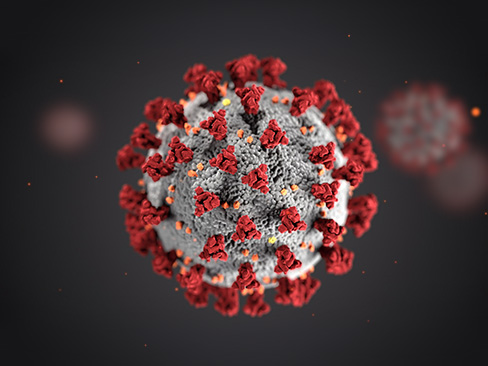
\includegraphics[width=0.4\textwidth]{Immagini/coronavirus.png}
	\caption{Molecola di un coronavirus}
	\label{fig:Amminoacido}
\end{figure}

All'interno dell'involucro troviamo una simmetria elicoidale dei nucleocapsidi, che in realtà è molto rara tra i virus a RNA a senso positivo. I CoV sono classificati nell'ordine Nidovirales, famiglia Coronaviriade e sotto famiglia Orthocoronavirinae. Nidovirales è un ordine di virus a RNA a singolo filamento positivo. Essi si distinguono da altri virus a RNA per la loro lunghezza e complessità del genoma e per la presenza di una struttura a corona di proteine sulla superficie virale. Il loro genoma contiene diversi geni che codificano proteine non strutturali coinvolte nella replicazione e nella trascrizione del virus nonché geni che codificano le proteine strutturali che costituiscono il virus stesso. Gli Nidovirales includono quattro famiglie virali:
\vspace{10pt}
\begin{itemize}
	\item Coronaviridae,
	\vspace{5pt}
	\item Arteriviridae,
	\vspace{5pt}
	\item Roniviridae,
	\vspace{5pt}
	\item Mesoniviridae.
\end{itemize}

La famiglia Coronaviridae è una famiglia di virus a RNA a singolo filamento positivo che causano malattie respiratorie e gastroenteriti in animali e in alcuni casi anche nell'uomo. I coronavirus sono stati scoperti per la prima volta negli anni '60, e devono il loro nome alla loro forma a corona, che deriva dalle protuberanze sulla loro superficie virale. La famiglia Coronaviridae è suddivisa in quattro generi:
\vspace{10pt}
\begin{itemize}
	\item Alphacoronavirus,
	\vspace{5pt}
	\item Betacoronavirus,
	\vspace{5pt}
	\item Gammacoronavirus,
	\vspace{5pt}
	\item Deltacoronavirus.
\end{itemize}

Un'analisi filogenetica ha inserito SARS-CoV2 sotto il sottogenere Sarbecovirus del genere Betacoronavirus. 

Le 4 proteine strutturali, citate in precedenza, sono richieste dalla maggior parte dei CoV per produrre una particella virale strutturalmente completa suggerendo che alcuni Cov possono codificare proteine aggiuntive con funzioni in sovrapposizione compensative.

\subsection{RNA polimerasi}\label{subsec:es_subsec}
%https://www.unisr.it/news/2020/7/rna-polimerasi-la-fotocopiatrice-distratta-di-sars-cov-2
La fase di ingresso del virus viene approfondita nella prossima sezione, ora pensiamo a cosa succede quando è all'interno. Una volta all'interno della parte acquosa della cellula ospite, chiamata citosol, il virus si "scompone" rilasciando il suo contenuto; un insieme di proteine e materiale genetico. L'uomo conserva l'informazione genetica, ovvero quella che ci permette di costruire le cellule, nelle molecole di DNA, il virus utilizza una singola molecola di RNA. L'RNA è presente anche nell'uomo, ma che principalmente viene utilizzato per la costruzione delle proteine. 

Una volta che il coronavirus ha infettato una cellula, il suo scopo è quello di far si che si costruiscano nuove copie dello stesso in modo da avere una discendenza in grado di espandere la specie. Tutto quello che è presente nella singola cellula infetta deve essere "copiato" e assemblato per formare nuovi vironi. Per ottenere la "copia" è necessario replicare il materiale genetico "RNA" del virus stesso. Il meccanismo che permette di far ciò si chiama RNA polimerasi, ovvero un enzima che è in grado di formare lunghe catene di RNA. In modo specifico l'RNA polimerasi di SARS-CoV-2 si chiama RdRP (RNA polimerasi RNA-dipendente). 

\begin{figure}
	\centering
	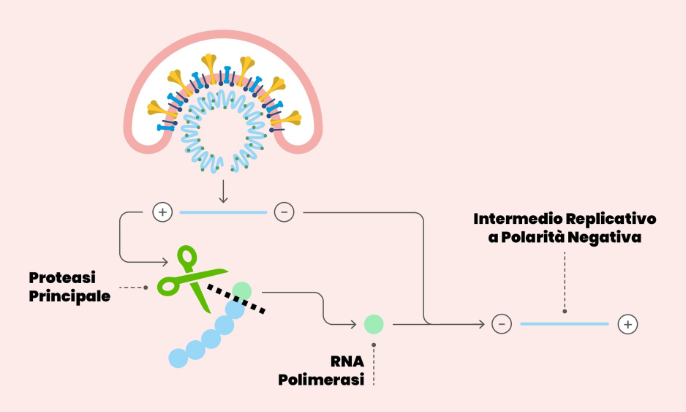
\includegraphics[width=0.6\textwidth]{Immagini/RNA_polimerasi.png}
	\caption{Principio del RNA polimerasi}
	\label{fig:Amminoacido}
\end{figure}

Esso viene però definito "distratto", infatti ogni volta che effettua la "copia" del materiale genetico originale commette degli errori, di conseguenza la copia presenta delle differenze. Le seguenti differenze non sono altro che mutazioni che si ripercuotono sulla struttura delle proteine del virus e sulla loro funzione. Non a caso si sono sentite varie varianti presenti come Delta, Omicron, etc... Quello che succede è che l'RNA polimerasi ha fatto una copia del genoma virale e ha cambiato una base di RNA. In ogni caso le mutazioni hanno conseguenze sul virus, possono essere neutre, vantaggiose o svantaggiose. Una mutazione può iniziare a circolare se essa da un vantaggio per il suo ciclo vitale, questo può significare essere più abile nell'infettare, ma provocare meno danni nell'organismo ospite, dato che un virus altamente letale è destinato a scomparire per mancanza di ospiti.

\section{Glicoproteina Spike}\label{sec:cap_sec_subsec}
%https://www.frontiersin.org/articles/10.3389/fimmu.2020.576622/full#f2
La glicoproteina spike svolge un ruolo essenziale nell'attaccamento, nella fusione e nell'ingresso del virus nella cellula ospite. Una caratteristica dei coronavirus è quella di accedere alle cellule ospiti e poi dare inizio all'infezione attraverso la fusione delle membrane virali alle cellule. La fusione della membrana viene mediata dalla membrana di tipo 1 della glicoproteina spike e dal recettore affine della cellula ospite. Essendo in una posizione superficiale nella struttura del virus, ciò la rende un bersaglio diretto per le risposte immunitarie dell'ospite rendendola anche il principale bersaglio degli anticorpi. Data la sua importanza nella replicazione e fusione virale è al centro della maggior parte delle strategie vaccinali e degli interventi terapeutici. 

La glicoproteina Spike viene sintetizzata come precursore di una poliproteina sul reticolo endoplasmatico ruvido (RER). Il precursore non processato ospita una sequenza segnale del reticolo endoplasmatico (ER) situato nel terminale N, che indirizza la glicoproteina alla membrana RER. Durante la sintesi vengono aggiunte catene laterali di oligosaccaridi ad alto contenuto di mannosio. Poco dopo la sintesi i monomeri della glicoproteina trimerizzano, il che può facilitare il trasporto dall'ER al complesso di Golgi. Il complesso di Golgi è un organulo di composizione lipo-proteica con una delicata struttura nella cellula in posizione paranucleare che si occupa di rielabolare, selezionare ed esportare i prodotti del reticolo endoplasmatico. All'interno del complesso di Golgi la glicoproteina spike viene scissa proteoliticamente dalla furina cellulare o da proteasi simili in S1 e S2. La subunità di superficie S1, che attacca il virus al recettore della superficie della cellula ospite e la subunità S2 che media la fusione delle membrane cellulari alla cellula ospite. Anche dopo la fase di scissione le subunità S1 e S2 rimangono associate attraverso interazioni non covalenti in uno stato di profusione metastabile. La scissione è però necessaria per l'infettività virale ed è anche necessaria per un efficacie infezione delle cellule polmonari. Un segnale di recupero dell'ER costituito da un motivo conservato KxHxx assicura che la proteina matura si accumuli vicino al compartimento intermedio di Golgi dove guidata dall'interazione con la proteina di membrana (M) partecipano all'assemblaggio delle particelle virali. Una frazione delle proteine mature viaggia attraverso via secretoria fino alla membrana plasmatica, dove può mediare la fusione di cellule infette con cellule non infette per formare cellule giganti multinucleate.

\subsection{Struttura della proteina e funzione}\label{subsec:es_subsec}
Come accenato nei precedenti paragrafi la glicoproteina spike svolge un ruolo fondamentale nell'infezione virale e nella patogenesi. Essa è un trimero fortemente glicosilato. La subunità S1 è composta da 672 amminoacidi ed organizzata in 4 domini: un dominio N-terminale; un dominio C-terminale, noto anche come dominio di legame; due sottodomini SD1 e SD2. Mentre la subunità S2 è composta da 588 amminoacidi e contiene un peptide di fusione idrofobica N-terminale, due ripetizioni eptade, un dominio transmembrana e una coda citoplasmatica.

Come una tipica proteina di fusione di classe I la glicoproteina spike condivide caratteristiche strutturali topologiche e meccaniche comuni con altre proteina di fusione di classe I come la glicoproteina dell'involucro dell'HIV e l'emoagglutinina del virus dell'influenza. Essa è una macchina coformazionale che media l'ingresso virale riorganizzando da uno stato non unliganded metastabile, attraverso uno stato intermedio ad uno stato post fusione stabile. Da quando è stata resa pubblica la struttura sono state scoperte numerose strutture per i frammenti di trimero della glicoproteina spike negli stati pre e post fusione. 

\begin{figure}
	\centering
	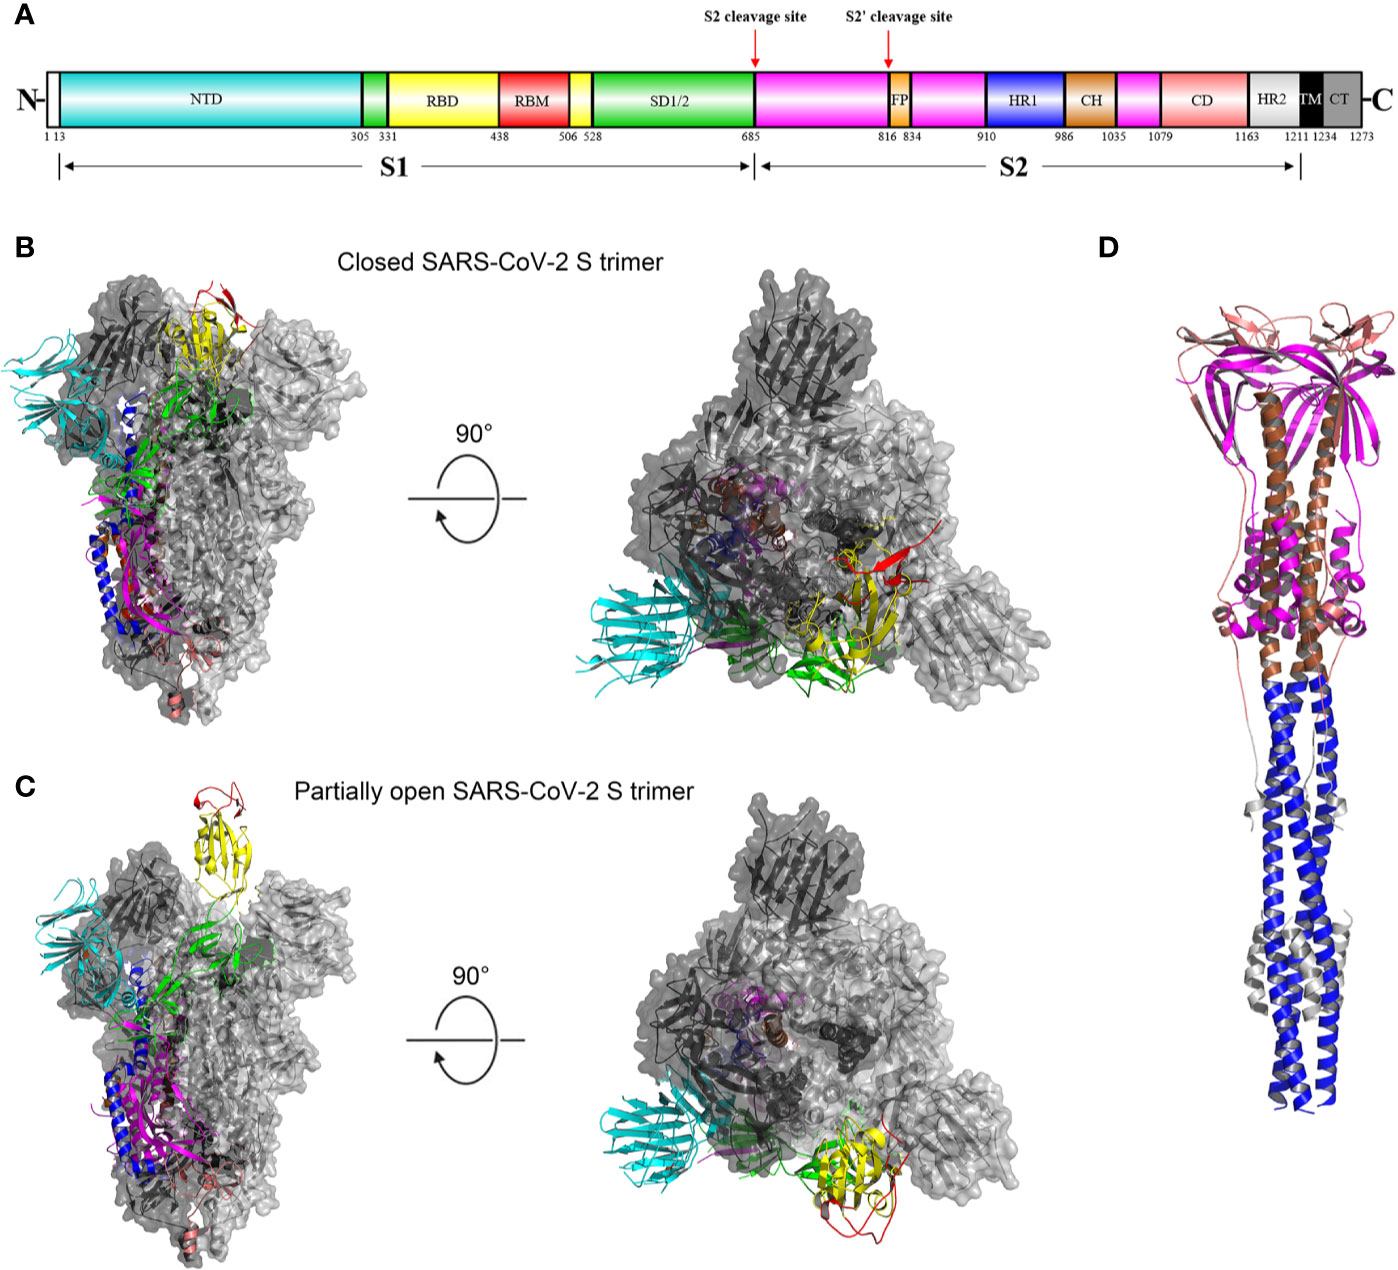
\includegraphics[width=0.7\textwidth]{Immagini/Composizione_strutturale.png}
	\caption{Struttura di massima della glicoproteina spike}
	\label{fig:StrutturaMassima}
\end{figure}

L'architettura di massima dell'ectodominio pre fusione della spike è stabilizzato da due mutazioni consecutive della prolina in due conformazioni determinate dalla microscopia crioelettronica a singola particella è un trimero con una sezione trasversale triangolare. La differenza strutturale tra queste due conformazioni risiede solo nella posizione di uno dei tre RDB. Quando tutti e tre gli RBD sono nella posizione giù il trimero risultante di ectodominio S assume una configurazione chiusa, in cui la superficie di legame del recettore dell'RBD S1 è sepolta tra i protomeri e non può essere accessibile dal suo recettore (Fig. \ref{fig:StrutturaCovid}B). Il trimero di ectodominio S con un singolo RBD nella posizione "up" assume una conformazione parzialmente aperta e rappresenta lo stato funzionale poiché la superficie di legame del recettore del RBD "up" può essere completamente esposta (Fig. \ref{fig:StrutturaCovid}C). La subunità S1 riposa mentre il trimero S2 stabilizzano quest'ultimo nella conformazione di pre fusione. Quando il trimero di ectodomionio adotta una conformazione parzialmente aperta l'RBD nella posizione "su" abolirà i contatti con la subunità S2 di un protomero adiacente, destabilizzando la conformazione parzialmente aperta. Ciò sarà vantaggioso per la dissociazione e faciliterà i riagganciamenti subiti per mediare l'ingresso virale. 

Le strutture di pre fusione del coronavirus umano senza due mutazioni consecutive della prolina rivelano solo una conformazione completamente chiusa. In particolare è noto che la pre fusione trimerica risiede principalmente in una configurazione chiusa che è conformazionalmente mascherata per eludere le neutralizzazioni mediate dagli anticorpi. Si può quindi pensare che le glicoproteine spike del covid-19 native su virioni maturi e infettivi che condividano una simile caratteristica di mascheramento conformazionale, nascondendo la superficie di legame del recettore.

\subsection{Scudo di glicani della glicoproteina spike}\label{subsec:es_subsec}
Come nominato in precedenza la proteina spike del SARS-CoV-2 è fortemente circondata da glicani N-legati che sporgono dalla superficie del trimero. Sono stati incontrati fino a 22 glicani N-legati che probabilmente svolgono un ruolo importante nel ripiegamento delle proteine e nell'invasione immunitaria dell'ospite come scudo glicano. Dei 22 potenziali disponibili per la glicosilazione, 14 vengono identificati come prevalentemente occupati da glicani di tipo complesso. I restanti invece risultano dominati da glicani di tipo oligomannosio che sono diversi da quelli fondati sulle glicoproteine dell'ospite. Per glicosilazione si intende una modifica della struttura della proteina da parte del complesso di Goigi, durante o in seguito ad un processo di sintesi proteica. Essa avviene per più motivi, uno dei quali è il raggiungimento del ripiegamento corretto, la può proteggere dall'attaccco di proteasi e aumenta la solubilità della molecola che viene dunque stabilizzata in tutti gli aspetti. Si può anche affermare che l'affinità di legame tra la proteina spike del SARS-CoV-2 e ACE2 non dipendono dalla glicosalinzione della stessa.

Quando i glicani specifici sono mappati sulla struttura di pre fusione dell'ectodominio della spike del SARS-CoV-2 il modello ha mostrato livelli sostanzialmente più elevati di superficie priva di glicani. Questo ci porta alla considerazione che la proteina spike del SARS-CoV-2 è ricoperta da uno scudo meno denso e quindi risulta essere una buona notizia per i potenziali vaccini. 

Nel caso di SARS-CoV-2, più recentemente è stato dimostrato che un potente anticorpo neutralizzante sia contro SARS-CoV che SARS-CoV-2, S309, riconosce un epitopo RBD contenente glicano altamente conservato. Queste osservazioni suggeriscono che le frazioni di carboidrati potrebberò essere immunogeniche ed evidenziano la necessità per gli immunogeni di mostrare i glicani importanti per il riconoscimento degli anticorpi neutralizzanti. Di conseguenza anche in questo caso è diventa fondamentale la ricerca in questo campo per i vaccini.

\section{RBD}\label{sec:cap_sec_subsec}
%https://www.ncbi.nlm.nih.gov/pmc/articles/PMC9581196/
Diverse linee di ricerca hanno stabilito che l'enzima di conversione dell'angiotesina 2 (ACE2) è un recettore di ingresso per SARS-CoV-2. Interazioni dettagliate tra il SARS-CoV-2 RBD e il suo recettore sono state rivelate da diverse strutture in ACE2. Come detto nella sezione precedente le subunità S1 e S2 sono responsabili del legame del recettore e della fusione della membrana. La subunità S1 è costituita da un dominio N-terminale e un dominio di legame o RBD. Nello stato di pre fusione, la proteina S esiste come omotrimero e subisce grandi cambiamenti conformazionali per controllare l'esposizione e l'accessibilità del RBD.Tutto questo avviene mediante un meccanismo di "su" e "giù", la differenza sta nel rendere accessibile o inaccessibile il recettore. La struttura del nucleo RBD quando è lagata ad ACE2 è costituita da un foglio $\beta$ antiparallelo a cinque filamenti intrecciati con eliche e anelli di collegamento corti. 
\begin{figure}
	\centering
	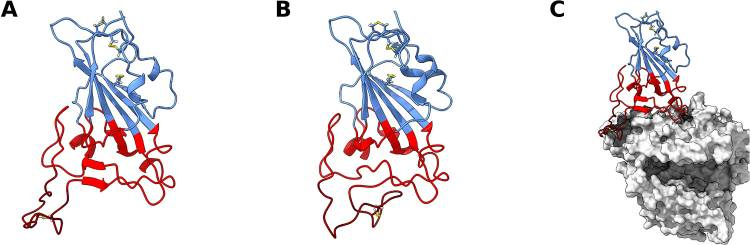
\includegraphics[width=0.7\textwidth]{Immagini/RBD_structure.png}
	\caption{Struttura del dominio di legame del recettore SARS-CoV-2, nella conformazione aperta (A) e chiusa (B). (C) rappresenta la struttura legata ad ACE2}
	\label{fig:RBDstructure}
\end{figure}

Questa struttura centrale del foglio $\beta$ è ulteriormente stabilizzata da 3 legami di di solfuro. Tra i filamenti centrali c'è una regione estesa contenente 2 filamenti $\beta$ corti, le eliche e gli anelli. Questa regione è il motivo legante il recettore (RBM) che contiene la maggior parte dei residui responsabili dell'interazione con ACE2. Quando complessato con ACE2, l'RBM si ripiega in una superficie concava che ospita l'$\alpha$-elica N-terinale di ACE2. E' proprio in questa superficie che diversi residui di RBM stabiliscono interazioni specifiche e non specifiche con i residui di ACE2. Dai dati disponibili riguardo alla struttura sembrerebbe che la struttura centrale sia abbastanza stabile, mentre l'RBM risulta molto dinamico e non definito strutturalmente, a meno che non sia legato ad altre proteine come ACE2. 

Durante il corso della pandemia sono state segnalate un numero significativo di mutazioni naturali della proteina Spike. Molte delle mutazioni sono state identificate nel RBD, alcune delle quali hanno dato origine a varianti virali. Si ritiene che molte di queste mutazioni RBD aumentino l'affinità di legame per ACE2 o riescono ad ingannare in modo migliore gli anticorpi monoclonali.  

I vaccini che sono stati elaborati nel corso della pandemia vanno proprio ad agire in questa zona tra RBD e ACE2, cercando di impedire che avvenga il contatto e che quindi impedire di conseguenza l'ingresso del virus all'interno dell'ospite.

\chapter{Obbiettivi}\label{chapter:obbiettivi}

%\Blindtext %Dummy Text - remove
\chapter{Progettazione}\label{chapter:progettazione}
%ecco qualche  commento.
%la sezione 4 richiede un po' di lavoro.
%manca tutto il livello di spiegazione tra l'introduzione e la sezione 4 attuale.
%in pratica devi raccontare in modo sintetico le strategie scelte (senza troppi dettagli
%implementativi), come hai organizzato le strutture di supporto
%e il perche'.
%Poi puoi raccontare lo pseudo codice, ma non nello stato attuale (riorganizzalo, semplificalo).
%Ci sta anche qualche disegno astratto sulla strategia di local search (puoi fare una griglia 2d
%che mostra il vicinato di traslazione o cose simili) ---> ?

%%% Sezione in cui spiegavo l'uso del biopython, causato dai file in ingresso che sono dei pdb
%%% Sezione sulle tecniche utilizate e le strutture dati che mi hanno aiutato all'interno del programma
%%% Poi avendo un approccio top-down spiego lo speudo codice
In questo capitolo viene affrontata la parte di implementazione e progettazione, vedremo le strategie di ricerca scelte, l'organizzazione delle strutture dati a supporto dell'esecuzione e poi avremo un approccio top-down verso il codice scritto. Introduco anche la libreria di supporto che ci ha permesso di svolgere il lavoro sul python.

\section{Librerie a supporto}\label{sec:libreriesupporto}  
In questo framework mi sono avvalso della libreria opensource \cite{BioPythonManual}. É una libreria di strumenti per la biologia computazionale e la bioinformatica. Essa contiene classi per rappresentare sequenze biologiche e annotazioni di sequenze ed è in grado di leggere e scrivere file provenienti da diversi formati. 
Questa libreria mi ha permesso di utilizzare il parser per i file pdb (Protein Data Bank) al cui interno sono codificate le informazioni riguardanti gli atomi come nome dell'atomo posizione all'interno dello spazio tridimensionale ed altre informazioni. Oltre a fornirmi un parser, al suo interno sono presenti dei moduli che permettono di generare oggetti come le catene, i residui e gli atomi stessi.
Questo da la possibilità di chiamare metodi specifici che semplificano il lavoro di gestione delle entità atomo, catena e residui. Viene fornita anche la possibilità di scrivere file in output nel formato desiderato (pdb), il che ci porta al secondo strumento utile il PyMOL. 

Il PyMOL è un opensuorce software di grafica 3D, che viene utilizzato per la rappresentazione di biomolecole. Come si può dedurre dalla parte iniziale del nomem si riferisce al linguaggio python. Risulta molto utile nella fase di verifica, ovvero quando si deve controllare ciò che è stato compiuto su una molecola. Fornisce un linguaggio di programmazione molto simile al python che permette di creare script per maneggiare e visionare le modifiche effettuate.
 
\section{Strategie di ricerca}\label{sec:Strategiediricerca}
All'interno di questo framework si è reso necessario utilizzare tecniche di ricerca locale nella fase in cui si cerca di andare a ristabilire il collegamento dei due loop alla parte mobile una volta effettuata una rotazione/traslazione su di essa. In questo caso la tecnica utilizzata è la hill-climbing, in cui si cerca di trovare il massimo (o il minimo) di una funzione di costo attraverso la ricerca di soluzioni vicine a quella corrente. In questo caso specifico, la funzione di ricerca cerca di ottimizzare la conformazione di un loop di collegamento alla volta attraverso la rotazione degli angoli torsionali. Si parte da una configurazione iniziale del loop rappresentata mediante ad una lista di residui, e cerco di migliorarla ruotando uno dei due angoli torsionali a disposizione, partendo da un residuo specificato. L'angolo torsionale viene scelto casualmente tra $\phi$ o $\psi$. Una volta applicata la rotazione viene restituita la nuova conformazione della proteina e si procede in questo modo fin tanto che non viene raggiunto il risultato desiderato. 

Viene utilizzata anche una tecnica di ricerca per guidare il processo che porta al completamento del percorso più breve tra le due configurazioni. La strategia di ricerca, in questo caso, è una forma di shortest path con una coda di priorità implementata tramite heap, albero binario ordinato. Essa viene utilizzata per selezionare il nodo con il costo totale (cioè il costo del percorso finora più la stima del costo rimanente) più basso in ogni iterazione. In questo modo si cerca di espandere i nodi che hanno costo totale più basso per primi. Ad ogni iterazione viene preso il vicinato del punto analizzato, si trasla in questi nuovi punti, come si può vedere in Fig. \ref{fig:Transizioni}. Per ogni transizione mediante un sistema di indici si risale ad un insieme di possibili rotazioni amiche, concetto che approfondiremo nelle sezioni successive, e dopodiché si prova la convergenza.

\begin{figure}[H]
	\centering
	\subfloat[][\emph{6 vicini}]
	{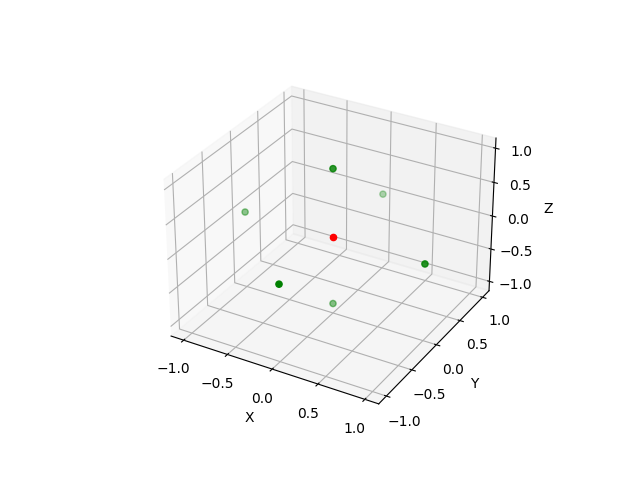
\includegraphics[width=0.5\textwidth]{Immagini/Transizioni_semplici.png}} 
	\subfloat[][\emph{26 vicini}]
	{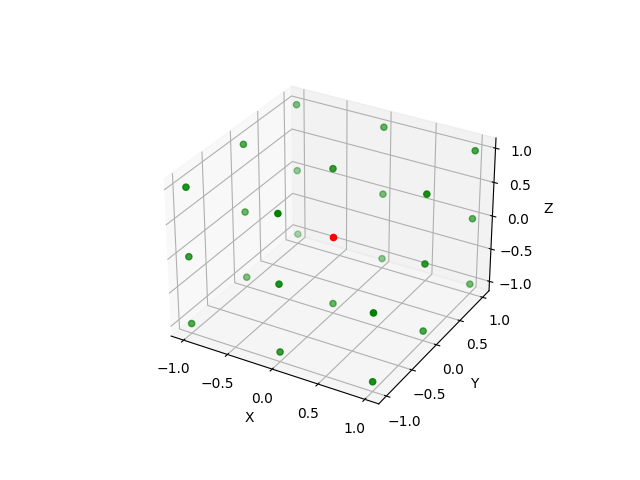
\includegraphics[width=0.5\textwidth]{Immagini/Transizioni_complesse.png}}
	\caption{In (\textbf{a}) vengono mostrati i 6 vicini come intorno del punto (0,0,0) contrassegnato di rosso; mentre in (\textbf{b}) vengono mostrati i 26 vicini di (0,0,0) contrassegnato sempre in rosso.}
	\label{fig:Transizioni}
\end{figure}

\section{Strutture dati a supporto}\label{sec:Strutturedati}
Le strutture dati sono importanti all'interno di un algoritmo, non solo per permettere di conservare informazioni, ma incidono anche sul tempo di esecuzione del singolo programma. Organizzare quindi l'accesso alle strutture dati nel modo migliore permette di risparmiare tempo d'esecuzione oltre a semplificare nella maggior parte dei casi la comprensione della stessa. 

Il linguaggio di programmazione scelto, python, necessità di studiare nel modo corretto come accedere alle strutture dati per evitare di trovarsi con dati inconsistenti poiché sono frutto di più modifiche. Per questo motivo e per quanto detto in precedenza io ho previsto 8 strutture di dati importanti: due dedicate a contenere la parte mobile e i loop, due dedicate al salvataggio delle posizioni acquisite da parte mobile e loop durante il cammino da una configurazione all'altra, due dedicate al salvataggio temporaneo e al ripristino in caso di clash delle coordinate dei loop pre e post rotazione, due dedicate alla gestione dei clash e due dedicate al concetto di amicizia delle matrici di rotazione pre-calcolate.

Le strutture dati sono state quasi tutte sviluppate come dei dizionari ad accesso chiave valore. Per quanto riguarda la struttura dati dedicata al controllo della presenza dei clash, la struttura contiene tuple di coordinate tridimensionali e per ciascuna tupla è contenuto la catena il residuo e l'atomo che si trovano in quella posizione. Questo è stato possibile mediante una discretizzazione di tutti gli atomi all'interno di una matrice tridimensionale. Chiaramente il passo di campionamento può essere impostato mediante costante, di default è impostato a 5 Ångström. \footnote{Ångström, sono un'unità di misura, non SI, pari a $10^-10m$.} 

Per quanto riguarda le strutture dati per mantenere salvate le coordinate dei loop e della parte mobile anch'esse sono organizzate come dizionari la cui chiave indicizza l'insieme delle varie coordinate. Le chiavi che indicizzano la struttura sono degli interi calcolati nel seguente modo:
$$
	key = x + y \cdot dx + z \cdot dx \cdot dy + r \cdot dx \cdot dy \cdot dz
$$
In questo caso $x, y, z$ identificano la traslazione che abbiamo effettuato sulla parte mobile, $r$ identifica univocamente la rotazione applicata alla parte mobile, mentre $dx, dy, dz$ sono le grandezze che su ogni asse separano la configurazione aperta da quella chiusa. Attraverso metodi di get e set possiamo settarli nelle variabili coinvolte nel processo evitando problemi di condivisione della memoria.

Abbiamo due dizionari dedicati al salvataggio temporaneo e al ripristino delle coordinate nel caso la rotazione non sia buona. Questi dizionari sono solamente per i due loop all'interno della funzione che si occupa di farli convergere alla parte mobile. La struttura dedicata ai loop e alla parte mobile invece sono due liste che a loro volta contengono residui a cui applicare le varie rotazioni. 

Le ultime due strutture dati nominate, utilizzate per il concetto di amicizia, sono a loro volta dei dizionari indicizzati per chiave, dove la chiave è appunto l'indice $r$ nominato in precedenza che identifica univocamente all'interno di queste strutture una matrice di rotazione e i suoi amici visti come una lista di indici.

Voglio comunque porre enfasi sullo studio necessario per progettare la singola struttura che mi ha concesso non solo di risolvere il problema della condivisione della memoria, ma anche di velocizzare il processo di accesso alla struttura dati e quindi portare più velocità nell'esecuzione della ricerca locale.

\section{Approccio Top-Down al codice}\label{sec:ApproccioTopDown}
Analizziamo lo pseudo-codice che permette di compiere il lavoro preposto dall'obbiettivo. 

\begin{algorithm}
	\caption{Inizializzazione framework}
	\label{alg:inizializzazione}
	\begin{algorithmic}
		\State $parser \gets PDBParser(PERMISSIVE=True, QUIET=True)$
		\State $covidchiusa \gets parser.getstructure(titleclosed)$
		\State $covidaperta \gets parser.getstructure(titleopen)$
		\State $calcoloamici(DIV)$
		\State $ptmob \gets partemobile(listacatene, catenainteresse)$
		\State $centroide \gets calcolocentroide(ptmob)$
		\State $normalizzazionestruttura(covidchiusa, covidaperta, centroide)$
		\State $calcoloparallelepipedo(covidchiusa, covidaperta)$
		\State $loop \gets identifyloop(listacatene, catenainteresse, costantiA)$
		\State $coil \gets [loop]$
		\State $loop \gets identifyloop(listacatene, catenainteresse, costantiB)$
		\State $loopr \gets loop[::-1]$
		\State $coil.append(loopr)$
		\State $salviamo(coildictcoordinates)$
		\State $key = x + y \cdot dx + z \cdot dx \cdot dy + r \cdot dx \cdot dy \cdot dz$
		\State $ptmob \gets partemobile(listacatene, catenainteresse)$
		\State $storedptmob \gets salviamo(ptmob)$
		\If{$key \notin posizioniacquisiteptmob$}
		\State $insert(posizioniacquisite, key)$
		\EndIf
		\State $residuipartefissa \gets partefissa(listacatene, catenainteresse)$
		\State $coordinate \gets salviamo(coildictcoordinates)$
		\If{$key \notin posizioniacquisiteloop$}
		\State $insert(posizioniacquisiteloop, key)$
		\EndIf
		\State $nuova\_chiave, prev \gets shortest\_path(key)$
		\State $printpdb(configurazioni)$
	\end{algorithmic}
\end{algorithm}

Come si può vedere in \ref{alg:inizializzazione} si vanno ad inizializzare le componenti principali del sistema. Innanzitutto viene creato un parser che ha il compito di parsare il file pdb in ingresso. Mediante il parser vengono estratte le configurazioni dai file pdb. Dopodiché vengono calcolate le matrici di rotazione e il concetto di amicizia tra matrici di rotazione, come riportato in \ref{subsec:amiciziarotazioni}. Una volta fatto, calcoliamo il centroide della parte mobile aperta e normalizziamo la struttura chiusa e aperta, in modo da averle centrate in (0,0,0). Dopodiché si restringe lo spazio di ricerca, come mostrato in \ref{subsec:areadiricerca}.

Una volta terminata la fase di inizializzazione, vengono presi i loop normalizzati, la parte mobile della configurazione chiusa normalizzata e la parte fissa utile per la gestione dei clash. Generiamo la chiave che ci permette di salvare le informazioni e cominciamo a cercare convergenza tra le due configurazioni mediante \ref{sec:shortestpath}.

\subsection{Amicizia tra matrici di rotazione}\label{subsec:amiciziarotazioni}

Utilizzando il metodo descritto in \ref{subsec:superfibonaccispiral}, si possono generare un insieme di vettori $x$ che rappresentano i vettori $x$ delle matrici di rotazione tridimensionale che verranno poi utilizzate per ruotare la parte mobile. 

Il concetto di amicizia tra due matrici è relativo al prodotto scalare tra i vettori $x$ e $y$ di due matrici. In questo caso è necessario definire delle soglie per discriminare una matrice piuttosto che un altra, le soglie impostate sono per quanto riguarda il prodotto scalare dei vettori $x$ $0.94$, mentre per i vettori $y$ $0.87$. Vengono impostate queste soglie poiché nel nostro caso il prodotto scalare dei vettori è compreso tra $[-1, +1]$, dove $+1$ rappresenta l'ugualianza dei due vettori, mentre $-1$ rappresenta la completa estraneità dei due vettori. 
Vengono scelte le seguenti soglie, perché vogliamo rendere piccolo lo spostamento da una matrice all'altra quando vengono applicate alla parte mobile; infatti, movimenti più piccoli garantiscono una migliore probabilità di convergenza tra i loop e la parte mobile. 

L'algoritmo proposto \ref{alg:calcoloamici} permette di ottenere il risultato mostrato in Fig. \ref{fig:Tagliox}, il parametro scelto è 20, che permette di generare 400 diversi vettori $x$ che a loro volta danno vita a 8000 matrici, in questo modo attraverso le soglie impostate in precedenza possiamo ottenere circa 3 o 4 migliaia di matrici amiche. 

\begin{figure}[H]
	\centering
	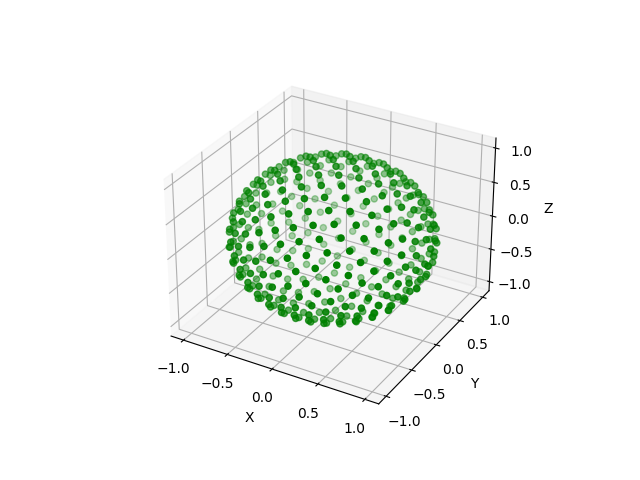
\includegraphics[width=0.6\textwidth]{Immagini/Tagliox.png}
	\caption{Punti equidistanti sulla superficie di una sfera, creando una distribuzione uniforme degli stessi.}
	\label{fig:Tagliox}
\end{figure}

\begin{algorithm}
	\caption{Procedura che permette il calcolo degli amici.}
	\label{alg:calcoloamici}
	\begin{algorithmic}
		\Procedure{calcoloamici}{$DIV$}
		\State $sphere \gets []$
		\State $n1 \gets DIV$
		\State $n \gets n1 * n1$
		\State $golden\_angle \gets 3.1415 \cdot (3 - \sqrt{5})$
		\For{$i$ \textbf{in} $range(n)$}
		\State $\theta \gets golden\_angle \cdot i$
		\State $pos \gets float(i / (n-1))$
		\State $z \gets (1-1.0/n-(1.0/n-1))\cdot pos+(1.0/n-1)$
		\State $radius \gets \sqrt{1 - z \cdot z}$
		\State $temp \gets [0, 0, 0]$
		\State $temp[2] \gets radius \cdot \cos(\theta)$
		\State $temp[1] \gets radius \cdot \sin(\theta)$
		\State $temp[0] \gets -z$
		\State $sphere.append(temp)$
		\EndFor
		\For{$x, j$ \textbf{in} $zip(sphere, range(len(sphere)))$}
		\State $multiplier \gets [0, 0, 1]$
		\If{$j == 0$}
		\State $multiplier \gets [0, 0, -1]$
		\EndIf
		\State $y \gets \langle x,multiplier \rangle$
		\State $y\_norm \gets normalizza(y)$
		\State $z \gets \langle x,y \rangle$
		\State $z\_norm \gets normalizza(z)$
		\For{$i$ \textbf{in} $range(DIV)$}
		\State $angle \gets radians((360/DIV*i))$
		\State $y_new \gets y_norm\cdot\cos(angle) - z\cdot\sin(angle)$
		\State $z_new \gets y_norm\cdot\sin(angle) + z\cdot\cos(angle)$
		\EndFor
		\EndFor
		\State $amici \gets amici(0.94, 0.87)$ 
		\EndProcedure
	\end{algorithmic}
\end{algorithm}

\subsection{Riduzione area di ricerca}\label{subsec:areadiricerca}
Restringere l'area di ricerca è fondamentale per non perdere tempo computazionale in zone dello spazio tridimensionale che non sono utili ai fini della ricerca. Per questo ho sviluppato la seguente funzione \ref{alg:parallelepipedo}.
\begin{algorithm}
	\caption{Calcolo del parallelepipedo}
	\label{alg:parallelepipedo}
	\begin{algorithmic}
		\Procedure{calcoloparallelepipedo}{$chiusa, aperta$}
		\State $mobilclosedpart \gets partemobile(listacatene, catenainteresse)$
		\State $mobilopenedpart \gets partemobile(listacatene, catenainteresse)$
		\State $ca \gets$ \Call{calcolocentoide}{$mobilopenedpart$}
		\State $cc \gets$ \Call{calcolocentoide}{$mobilclosedpart$}
		\State $x\_parallelepipedo\_min \gets$ \textit{int}$(min(0,(ca[0]-cc[0])-1))$
		\State $x\_parallelepipedo\_max \gets$ \textit{int}$(max(0,(ca[0]-cc[0])+1))$
		\State $y\_parallelepipedo\_min \gets$ \textit{int}$(min(0,(ca[1]-cc[1])-1))$
		\State $y\_parallelepipedo\_max \gets$ \textit{int}$(max(0,(ca[1]-cc[1])+1))$
	    \State $z\_parallelepipedo\_min \gets$ \textit{int}$(min(0,(ca[2]-cc[2])-1))$
		\State $z\_parallelepipedo\_max \gets$ \textit{int}$(max(0,(ca[2]-cc[2])+1))$
		\State $dx \gets x\_parallelepipedo\_min - x\_parallelepipedo\_max$
		\State $dy \gets y\_parallelepipedo\_min - y\_parallelepipedo\_max$
		\State $dz \gets z\_parallelepipedo\_min - z\_parallelepipedo\_max$
		\EndProcedure
	\end{algorithmic}
\end{algorithm}
In questo modo riusciamo a restringere il campo di lavoro, ad una sorta di parallelepipedo che contiene entrambe le configurazioni. Il parallelepipedo è individuato dalle coordinate per ogni asse massime e minime e dopodiché possiamo verificare l'appartenenza all'interno dello stesso mediante una semplice funzione che verifica l'appartenza. All'interno di questa funzione vengono anche calcolati gli indici che permettono di calcolare la chiave di indicizzazione di ogni nodo generato.  

\section{Shortest-Path}\label{sec:shortestpath}
Come descritto in \ref{chapter:obbiettivi}, l'obbiettivo è quello di convergere tra la conformazione chiusa e quella aperta mediante il cammino con il minor costo possibile.
Per fare ciò lavoriamo e ci concentriamo esclusivamente sulla conformazione chiusa, l'utilizzo della conformazione aperta è esclusivamente necessario per verificare il raggiungimento dell'obiettivo. 

Terminando la fase di inizializzazione in \ref{alg:inizializzazione}, si procede nel individuare e salvare i loop, che mettono in collegamento la parte mobile con la parte fissa. I due loop sono simili, ma diversi nella direzione da loro presa, ovvero il loop-A si dirige dalla parte fissa alla parte mobile, mentre il loop-B lavora al contrario quindi per rendere omogeneo il comportamento del programma nei confronti dei due loop è necessario capovolgere il secondo. Questo non comporta nessun altra modifica, è però necessario ricordarsi di capovolgere il loop nel momento in cui si effettua il processo di scrittura file. Le costanti sul posizionamento dei loop sono state fornite insieme alle configurazioni ed è importante sottolineare che è stato preso un residuo in più in capo e in coda al loop, per verificare che ogni modifica si adatti bene alla struttura a cui si deve attaccare. Una volta che abbiamo terminato l'attività di salvataggio dei loop e della parte mobile avviamo shortest-path \ref{alg:algoritmoshortpath} e una volta concluso stampiamo passo passo le configurazioni intermedie. 

\begin{algorithm}
	\caption{Shortest-Path}
	\label{alg:algoritmoshortpath}
	\begin{algorithmic}
		\Procedure{Shortest-path}{$start\_idx$}
		\State $heap \gets [(0, start\_idx)]$
		\State $prev \gets \{\}$, $costo \gets \{\}$
		\State $prev[start\_idx] \gets -1$, $costo[start\_idx] \gets 0$
		\While {heap}
		\State $cost, indice\_current \gets heap$
		\State $movimento, r \gets indice\_current$
		\State $ptmob \gets load(indice\_current)$, $loop \gets load(indice\_current)$
		\State $friends \gets amici(r)$
		\For {$traslazione$ \textbf{in} $traslazioni$}
		\For {$r2$ \textbf{in} $friend$}
		\State $ptmob \gets load(r2)$, $ptmob \gets applytransition(traslazione)$
		\If {\textbf{not} $is\_allowed(ptmob)$}
		\State \textbf{continue}
		\EndIf
		\State $pre-processing(ptmob)$
		\State $convergenza \gets esecuzione\_rotazioni()$
		\If {$convergenza$}
		\State $nuovo\_indice \gets indice\_current$
		\State $nuovo\_costo \gets costo + costo(r, r2)$
		\If {$nuovo\_costo < costo[indice\_current]$}
		\State $prev[nuovo\_indice] \gets indice\_current$, 
		\State $costo[nuovo\_indice] \gets nuovo\_costo$
		\State $heap \gets (nuovo\_indice, nuovo\_costo)$
		\State $insert(posizioniacquisiteloop, nuovo\_indice)$
		\State $insert(posizioniacquisiteloop, nuovo\_indice)$
		\If {$dist(ptmob, covid\_aperta) < 0.1$}
		\State \textbf{return} $nuovo\_indice, prev$
		\EndIf
		\EndIf
		\EndIf 
		\EndFor
		\EndFor
		\EndWhile 
		\EndProcedure
	\end{algorithmic}
\end{algorithm}
Come descritto in \ref{alg:algoritmoshortpath}, viene utilizzata una coda di priorità implementata tramite heap, albero binario ordinato, in cui passo passo vengono inseriti i nuovi nodi scoperti. Si inizia iterando sulla struttura dati, e si estrae il nodo che ha costo minore. Una volta estratto il nodo, prendiamo l'indice e ne ricaviamo la traslazione che fino a quel momento ci ha permesso di arrivare in quella posizione e la rotazione della parte mobile. Recuperiamo e settiamo nuovamente le coordinate alla parte mobile e ai loop, in modo tale da ripartire da dove eravamo rimasti. Una volta estratte le rotazioni amiche dell'attuale, si cercano nuove soluzioni. 

Per ogni traslazione elencate nell'array traslazioni, come in Fig. \ref{fig:Transizioni}, e per ogni rotazione amica si cerca convergenza. Prima di raggiungere se possibile la convergenza è necessario effettuare delle operazioni, ovvero dobbiamo caricare la parte mobile nella determinata rotazione $r2$ poiché tutte le rotazioni sono pre-calcolate in modo da ridurre il tempo di esecuzione; dobbiamo traslare la parte mobile nella corretta posizione fornita dagli indici. Una volta posizionata correttamente la parte mobile è necessario effettuare il controllo che la parte mobile sia all'interno del parallelepipedo, per i motivi descritti in \ref{subsec:areadiricerca}, dopodiché se la rotazione è consentita dobbiamo effettuare il pre-processing per determinare le strutture che permettono di comprendere la presenza di clash quando si ruotano i residui che compongono i loop. 

Terminata la fase di pre-processing necessaria all'individuazione di clash, si procede alla convergenza, ovvero si cerca di far convergere i loop alla nuova posizione della parte mobile, vedremo più nel dettaglio questa funzione nella prossima sottosezione. Se viene raggiunta convergenza, nella maggior parte dei casi è cosi perché gli spostamenti sono relativamente piccoli a meno di clash insormontabili, va inserito all'interno dell'heap il nuovo nodo se e soltanto se il nuovo costo è migliore del costo già presente per quel nuovo indice nel dizionario dei costi. Il nuovo costo viene calcolato come descritto in \ref{subsec:calcolocostoarco}. Se effettivamente minore inseriamo il nuovo costo ed è anche necessario aggiornare anche il nodo precedente che ci ha permesso di arrivare a questo nodo nella struttura prev. 

Se abbiamo raggiunto convergenza è necessario poi salvare le nuove coordinate sia dei loop che della parte mobile. É importante anche capire se abbiamo ottenuto il nostro obbiettivo principale ovvero se siamo arrivati a convergenza tra le due configurazioni, quella attuale e quella aperta, per fare ciò utilizziamo semplicemente la distanza euclidea tra la configurazione attuale e quella di arrivo. La soglia impostata per terminare il lavoro è 0.1 A che garantisce l'effettiva convergenza. 

\subsection{Calcolo costo arco}\label{subsec:calcolocostoarco}
La parte più importante all'interno dell'algoritmo di shortest-path è quello di calcolare il costo del nodo che si sta analizzando. Il nostro costo viene calcolato mediante 3 contributi: il primo è il costo del movimento delle coordinate; il secondo è costo dell'amicizia tra le matrici di rotazione; il terzo è lo spostamento dall'asse centrale che supponiamo essere il percorso migliore.

Analizzando nel dettaglio le componenti troviamo che il costo del puro movimento è costante a 1, poiché che ci si muova in negativo o in positivo il delta di spostamento è 1 a patto che venga utilizzato il vicinato di transizione semplice (Fig. \ref{fig:Transizioni} \textbf{a}). 

Il costo dell'amicizia tra due matrici è estratto come prodotto scalare dei due vettori $x$ e $y$, però preso in questo modo, ovvero $(1-\langle x, x2\rangle) + (1-\langle y, y2\rangle)$. In questo il costo di amicizia ci permette di pagare poco se ci muoviamo poco, mentre pagare un costo elevato se decidiamo di effettuare un movimento elevato. 

Il terzo componente è dedicato alla distanza del nuovo centroide generato dal segmento, ovvero se ci allontaniamo dall'ipotetico percorso migliore paghiamo una penalità. Questo coefficente viene calcolato come la distanza tra un punto e un segmento usando la proiezione ortogonale del punto sul segmento e la distanza euclidea tra il punto originale e il punto proiettato sul segmento.

Queste tre componenti determinano il costo del nuovo nodo generato, privilegiando i nodi più vicini al percorso ottimale e lasciando lo sviluppo dei nodi pù marginali in fondo.

\subsection{Convergenza tra loop e parte mobile}\label{subsec:convergenza}
\begin{algorithm}
	\caption{Esecuzione rotazioni tra loop e parte mobile}
	\label{alg:algconvergenza}
	\begin{algorithmic}
		\Procedure{esecuzione\_rotazioni}{ptmob}
		\State $distanza\_iniziale \gets [0,0]$
			\For{$loop$ \textbf{in} $coil$}
		\State $distanza\_iniziale[idx] \gets$ \Call{objective\_function}{$loop$, $ptmob$}
		\EndFor
		\State $angle\_to\_direction \gets$ \Call{suggestedsetofangle}{180, 1}
		\For{$a$ \textbf{in} $angle\_to\_direction$}
			\For{$loop$ \textbf{in} $coil$}
				\If{($distanza\_iniziale[idx] \geq 0.1000$)}
					\State $res \gets$ \textit{int}(\textit{len}($loop$)) $-$ 2
					\State $prova \gets$ \Call{hillclimbing}{$loop$, $residui\_costanti[idx]$, $a$, $res$}
					\State $distance \gets$ \Call{objective\_function}{$prova$, $ptmob$}
					\If{($distance < distanza\_iniziale[idx]$)}
						\State $clash \gets$ \Call{searchneighbor}{$prova$}
						\If {\textbf{not} ($clash$)}
							\State $distanza\_iniziale[idx] \gets distance$
							\State $storage(prova, idx)$
						\EndIf
					\EndIf
				\EndIf
				\State $load(loop, idx)$
			\EndFor
		\EndFor
		\For {$i$ \textbf{in} \textit{range}(iterazioni\_massime)}
		\For{$loop$ \textbf{in} $coil$}
		\If {\textbf{not} stop\_loop[idx]}
		\State $stop\_loop[idx] \gets$ \Call{stopsearch}{}
		\If{($distanza\_iniziale[idx] \geq 0.1000$)}
		\State $n\_res \gets$ \Call{suggestedresidue}{\textbf{len}(loop)}
		\State $angle \gets$ \Call{suggestedangle}{distanza\_iniziale[idx]}
		\State $swap \gets$ \Call{suggestedchange}{distanza\_iniziale[idx]}
		\State $loop\_new \gets$ \Call{hillclimbing}{$loop$, $residui\_costanti[idx]$, $angle$, $n\_res$}
		\State $distance \gets$ \Call{objective\_function}{$loop\_new$, $ptmob$}
		\If{($distance < distanza\_iniziale[idx]$)}
		\State $clash \gets$ \Call{searchneighbor}{$prova$}
		\If {\textbf{not} ($clash$)}
		\State $distanza\_iniziale[idx] \gets distance$
		\State $storage(prova, idx)$
		\EndIf
		\EndIf
		\State $load(loop, idx)$
		\EndIf
		\EndIf
		\EndFor
		\EndFor
		\If {$distanza\_iniziale[0] \leq 0.1$ \textbf{and} $distanza\_iniziale[1] \leq 0.1$}
		\State \textbf{return} \textit{True}
		\EndIf
		\State \textbf{return} \textit{False}
		\EndProcedure
	\end{algorithmic}
\end{algorithm}

La parte più importante è appunto questa che si occupa della convergenza dei loop, verso la nuova conformazione della parte mobile. Innanzitutto viene calcolata la distanza che i loop devono colmare fra se stessi e i punti di aggancio della parte mobile, che avviene mediante la funzione $objective\_function$(\ref{subsubsec:funzionetarget}). 

Una volta misurata la distanza da colmare, effettuando vari test, ho riscontrato che è possibile dare una mano alla convergenza dei loop, praticando delle rotazioni preliminari su un ampio spettro di angoli da $\ang{-180}$ a $\ang{180}$ con passo di campionamento $1$. Ogni angolo viene provato per ciascun angolo torsionale. Per effettuare la singola rotazione utilizziamo la funzione $hillclimbing$(\ref{subsubsec:hillclimbing}). Una volta effettuata la singola rotazione e propagata all'interno del loop è necessario, se la distanza risultante è minore della precedente si procede a verificare la presenza di clash per garantire la stabilità della proteina. 

Tutto ciò avviene grazie alla funzione $searchneighbor$(\ref{subsubsec:ricercavicini}), che si avvale di ciò che è stato fatto durante il pre-processing descritto in precedenza. Se non vengono riscontrati clash, la rotazione viene considerata valida e vengono aggiornate le coordinate nelle strutture dati a supporto dell'esecuzione.

Una volta terminata la fase di applicazione di queste rotazioni canoniche, si passa alle iterazioni che lavorano di fino in base alla distanza del loop. Come prima cosa ci si chiede se questo loop è stato fermato nella sua progressione perché, se è cosi non ha senso continuare a iterare se almeno uno dei loop non può raggiungere la meta. Se il loop non è ancora stato fermato verifichiamo che al giro successivo non debba essere fermato mediante la funzione $stopsearch$. Questa funzione agisce sulle distanze raggiunte nel corso delle iterazioni dal loop e calcola un indice di incremento tra le ultime 20 distanze raggiunte. Questo indice è sicuramente negativo perché la distanza decresce, se però è maggiore di $-0.01$ significa che la distanza raggiunta nel corso delle 20 distanze ha una differenza che è troppo piccola per proseguire il lavoro. Ovviamente ho eseguito vari test per trovare la soglia e il numero di distanze da prendere in considerazione ed ho cercato il miglior compromesso per evitare di fermare troppo presto il cammino del loop. 

Se il loop non è stato fermato allora devono essere determinati alcuni parametri: il residuo su cui lavorare, che viene determinato in modo casuale; l'angolo con cui provare la successiva rotazione determinato dalla funzione $suggestedangle$(\ref{subsubsec:suggerimentoangoli}); lo swap che interviene per cercare di smuovere il processo di convergenza del loop nel caso si raggiunga un "asintoto". Nel caso in cui venga richiesto uno swap, si effettuano delle rotazioni di $\ang{-0.5}$ e $\ang{0.5}$ sulla base del loop per smuovere il processo. Una volta effettuata la singola rotazione e propagata all'interno del loop è necessario, se la distanza risultante è minore della precedente, verificare la presenza di clash per garantire la stabilità della proteina.

Le iterazioni possono terminare per i seguenti motivi:
\vspace{10pt}
\begin{itemize}
	\item entrambi i loop raggiungono la distanza minima quindi la funzione restituisce l'avvenuta convergenza;
	\vspace{5pt}
	\item uno dei loop è stato fermato durante il processo di convergenza, quindi la funzione restituisce che la convergenza non è avvenuta;
	\vspace{5pt}
	\item uno dei due loop non ha colmato la distanza, quindi la convergenza non è avvenuta.
\end{itemize}

\subsubsection{Funzione obbiettivo}\label{subsubsec:funzionetarget}
La funzione obiettivo, \ref{alg:funzioneobj}, viene utilizzata per calcolare la distanza tra l'ultimo residuo del loop e la parte di attacco della parte mobile corrispondente. La distanza viene misurata mediante due contributi: il primo deriva dalla distanza euclidea dei due atomi carbonio $\alpha$; il secondo contributo è dato dal prodotto scalare dei due vettori tra gli atomi carbonio e azoto dell'ultimo residuo della parte mobile e del loop. 

É necessario considerare il prodotto scalare tra i due vettori, poiché è necessario che i due residui interagiscano nel modo corretto; infatti, i due atomi carbonio $\alpha$ potrebbero essere a contatto, ma i due atomi di carbonio e azoto potrebbero essere opposti e non favorire il legame tra i due residui. 
 
\begin{algorithm}
	\caption{Objective Function}
	\label{alg:funzioneobj}
	\begin{algorithmic}
		\Function{objective\_function}{$loop, ptmob$}
		\State $residuo\_loop \gets loop[resiude]$
		\State $residuo\_ptmob \gets ptmob[residue]$
		\State $distanzaCA \gets residuo\_loop[CA] - residuo\_ptmob[CA]$
		\State $asse\_loop \gets residuo\_loop[N] - residuo\_loop[C]$
		\State $asse\_loop \gets normalizza(asse\_loop)$
		\State $asse\_ptmob \gets residuo\_ptmob[N] - residuo\_ptmob[C]$
		\State $asse\_ptmob \gets normalizza(asse\_ptmob)$
		\State $prodotto\_scalare \gets \langle asse\_loop, asse\_ptmob \rangle$
		\State $product \gets (\sqrt{1-prodotto\_scalare}/2)$
		\State \textbf{return} $distanzaCA \cdot (1 + product)$
		\EndFunction
	\end{algorithmic}
\end{algorithm}

\subsubsection{Hillclimbing}\label{subsubsec:hillclimbing}
La funzione $hillclimbing$, \ref{alg:hillclimbing}, viene utilizzata per applicare il movimento ad un residuo e poi propagarlo al resto del loop. A seconda dell'angolo torsionale estratto necessitiamo di generare una matrice di rotazione differente. Nel caso $0$, ovvero $\phi$, costruiamo la matrice di rotazione sull'asse degli atomi C$\alpha$-N; nel caso $1$, ovvero $\psi$, costruiamo la matrice di rotazione sull'asse degli atomi C$\alpha$-C. Una volta calcolata la matrice la applichiamo ai residui a partire da quello scelto in modo randomico in precedenza. E' necessario controllare nel caso del loop-A di non applicare la rotazione in alcuni particolari residui che fanno parte del $\beta$-foglietto rigido. 
\begin{algorithm}[H]
	\caption{Hillclimbing}
	\label{alg:hillclimbing}
	\begin{algorithmic}
		\Function{hillclimbing}{$loop, angolo, idx\_rex$}
		\State $torsional\_angle \gets random(0,1)$
		\State $loop\_new \gets []$
		\If {$torsional\_angle == 0$}
		\State $asse \gets loop[idx\_rex][CA] - loop[idx\_rex][N]$
		\State $asse \gets normalizza(asse)$ 
		\State $rotation\_matrix \gets matrice(asse, angolo)$
		\Else
		\State $asse \gets loop[idx\_rex][CA] - loop[idx\_rex][C]$
		\State $asse \gets normalizza(asse)$ 
		\State $rotation\_matrix \gets matrice(asse, angolo)$
		\EndIf
		\For {$i$ \textbf{in} \textit{range}(0, idx\_rex)}
		\State $loop\_new \gets loop[i]$
		\EndFor
		\For {$i$ \textbf{in} \textit{range}(idx\_rex, \textit{len}(loop))}
		\State $loop\_new \gets ruota(loop[i])$
		\EndFor 
		\State \textbf{return} $loop\_new$
		\EndFunction
	\end{algorithmic}
\end{algorithm}
\subsubsection{SearchNeighbor}\label{subsubsec:ricercavicini}
La funzione $searchneighbor$, \ref{alg:searchnei}, si occupa di verificare la presenza di clash, ovvero interazioni tra atomi come descritto in \ref{subsec:ramachandranPrinciple}. In questo caso è necessario verificare sia che siano presenti clash tra i due loop, poiché sono a stretto contatto, e sia che siano presenti con gli altri atomi presenti nella proteina. L'unico modo per verificare la presenza di un clash è quella di controllare che la distanza euclidea tra due atomi sia maggiore rispetto alla somma dei rispettivi raggi di van der Walls.  
\begin{algorithm}[H]
	\caption{Searchneighbor}
	\label{alg:searchnei}
	\begin{algorithmic}[1]
		\Procedure{searchneighbor}{$residuo$}
		\State $res_linked \gets []$
		\If{$residue.id[1] \in side_chain_processed[idx_loop]$}
			\State $res_linked \gets side_chain_processed[idx_loop][residue.id[1]]$
		\EndIf
		\For{atom \textbf{in} residue}
			\If{atom.id \textbf{in} res\_linked}
				\For{atom\_check \textbf{in} res\_linked[atom.id]}
					\State $d \gets (atom\_check - atom)$
					\State $r \gets raggio(atom\_check)+raggio(atom)$
					\If{d $<$ r}
						\State \textbf{return} \textbf{True}
					\EndIf
				\EndFor
			\EndIf
			\State coordinate $\gets$ atom.get\_coord()
			\State key $\gets$ $(mx, my, mz)$
			\State six\_coord $\gets$ catch\_coordinates(key)
			\For{coord \textbf{in} six\_coord}
				\For{element \textbf{in} tridimensional\_clash[coord]}
					\State chain $\gets$ element['chain']
					\State atom\_to\_analize $\gets$ element['atom']
					\If{\textbf{not} same(atom, chain, residue)}
						\State $d \gets (atom\_to\_analize - atom)$
						\State $r \gets (raggio(atom\_to\_analize)+raggio(atom)$
						\If{d $<$ r}
							\State \textbf{return} \textbf{True}
						\EndIf
					\EndIf
				\EndFor
			\EndFor
		\EndFor
		\State \textbf{return} \textbf{False}
		\EndProcedure
	\end{algorithmic}
\end{algorithm}
\subsubsection{Suggestedangle}\label{subsubsec:suggerimentoangoli}
La funzione $suggestedangle$, \ref{alg:suggestedangle}, mi permette di determinare un angolo a partire dalla distanza residua. Questa funzione mi permette di avere un angolo piccolo quando la distanza è molto piccola e un angolo abbastanza grande quando la distanza è elevata(Fig. \ref{fig:fundis}). 

\begin{figure}
	\centering
	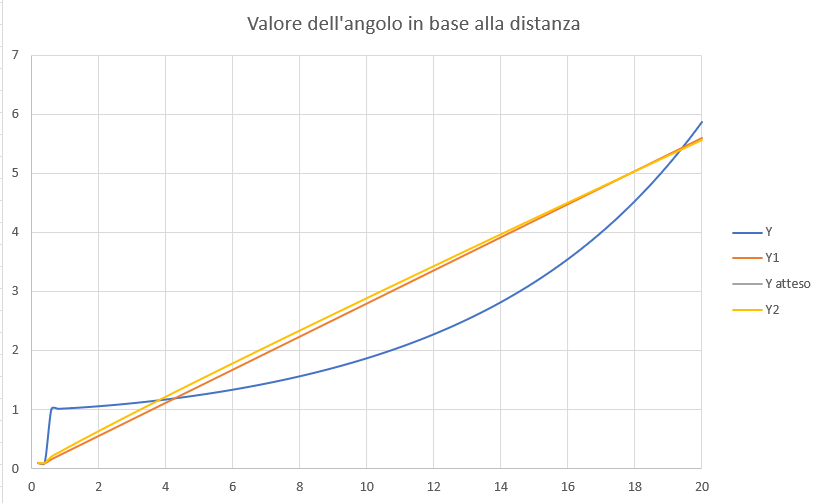
\includegraphics[width=0.6\textwidth]{Immagini/Funzionedistanza.png}
	\caption{La funzione Y2 è quella che mi permette di descrivere meglio il comportamento richiesto.}
	\label{fig:fundis}
\end{figure}

\begin{algorithm}
	\caption{SuggestedAngle}
	\label{alg:suggestedangle}
	\begin{algorithmic}
		\Function{suggestedangle}{$distanza$}
		\State $angle \gets 0.1$
		\If {$distanza \geq 0.5$}
		\State $angle \gets (2^{distanza^{-0.1}}\cdot distanza/6)$
		\EndIf
		\State \textbf{return} $angle$
		\EndFunction
	\end{algorithmic}
\end{algorithm}
\chapter{Risultati}\label{chapter:res}
%\Blindtext %Dummy Text - remove
%
%
%%%% Le Conclusioni
\pagestyle{plain}
\chapter*{Conclusione} %Se si cambia il Titolo cambiare anche la riga successiva così che appia corretto nell'conclusione
\addcontentsline{toc}{chapter}{Conclusione} %Per far apparire Introduzione nell'indice (Il nome deve rispecchiare quello del chapter)
Conclusione che riassume il lavoro svolto ed eventuali lavori futuri.

%\blindtext %Dummy Text - remove
%\blindtext %Dummy Text - remove
%
%%%% La bibliografia
\bibliographystyle{apalike} %{plain} -- Scegliere lo stile preferito
\cleardoublepage
\addcontentsline{toc}{chapter}{\bibname}
\bibliography{./Bibliografia}
%
\chapter*{Ringraziamenti}
Innanzitutto voglio ringraziare il Professor Alessandro Dal palù che mi ha assistito durante tutto questo percorso e mi ha permesso di raggiungere questo traguardo. La ringrazio non solo per la cordialità e la pazienza che mi ha dimostrato, ma anche per avermi concesso la possibilità di mettere in pratica ciò che studiato in questi anni lavorando al progetto "Carriere studenti". Voglio ringraziare anche il Professor Pietro Cozzini e Federica Agosta senza i quali sarei ancora a cercare di capire com'è fatta la catena laterale di un amminoacido.

Un grazie immenso alla mia famiglia perché se tutto ciò sta avvenendo è anche grazie a voi. Mamma scusami per tutte le volte che ti risposto male e trattato peggio forse non sono molto bravo a gestire la pressione, però senza di te non ce l'avrei fatta. Papa se sono un minimo determinato a raggiungere i miei obbiettivi è grazie a te che mi hai insegnato a non mollare mai e non dare nulla per scontato, spero di continuare cosi e non mollare mai come fai tu. Let'z ce ne sarebbero troppe da dire, ma per qualsiasi cosa ti servirà ci sarò sempre, in fin dei conti siamo fratelli. 

Alexa, da un anno e mezzo a questa parte i nostri cammini si sono intrecciati e fino ad ora tra alti e bassi è stato bellissimo; speriamo di poter condividere ancora tante altre avventure insieme. Grazie per essermi stata accanto sempre anche se so che non è stato facile.

Grazie a tutti i miei amici, quelle persone che ci sono sempre e che sempre ci saranno. Voglio però citare alcune persone in particolare con cui sono più legato nell'ultimo periodo, nonostante siate tutti molto importanti. Partendo da questi otto scappati di casa il cui unico obbiettivo è vandalizzarmi casa se salto un uscita. Ci sono però anche tanti bei momenti e notti magiche che non si possono dimenticare. Fede anche a te va un ringraziamento speciale per avermi ascoltato e tante volte risolto problemi che dal mio punto di vista sembravano insormontabili, la mia collega preferita. Marti, cosa possiamo dire, la mia seconda sorella aggiunta che ha passato un intero pomeriggio con me a guardare i legami covalenti, per non parlare di quella bellissima paperella gialla. Un ringraziamento speciale va anche a tutte quelle persone con cui ho condiviso questo percorso sia la triennale che la magistrale, abbiamo condiviso tanto tempo insieme e tanta sofferenza, teniamoci in contatto perché siamo un bel gruppo. Ci sono poi gli amici di una vita per cui non ci sono parole. 

Voglio ringraziare anche la mia classe di inglese che mi ha ascoltato durante tutte le lezioni e un grazie anche alla mia favorite teacher Kim che mi sta insegnando l'inglese con tanta pazienza perché diciamocelo non sono uno studente modello e si sa i compiti di inglese non vorrebbe farli nessuno.

Grazie a tutti.
%
% Le appendici
%\appendix
%\chapter{Appendice di Esempio}
\Blindtext
%
\end{document}